\documentclass[11pt,a5paper,oneside,openany]{scrreprt}

% -----------------------------------------------------------------------------
% Professional, restrained lecture-note design
% -----------------------------------------------------------------------------
\usepackage[T1]{fontenc}
\usepackage[scale=1.06,looser]{newtxtext}
\usepackage[scaled=0.92]{helvet}
\usepackage{microtype}
\usepackage{geometry}
\geometry{top=18mm,bottom=20mm,left=17mm,right=17mm,headheight=14pt}
\usepackage{setspace}
\setstretch{1.24}
\usepackage{mathtools,amsthm,bm}
\usepackage{newtxmath}
\usepackage{booktabs,tabularx,longtable,array,multirow}
\usepackage{enumitem}
\usepackage{xcolor}
\usepackage[most]{tcolorbox}
\usepackage{tikz}
\usepackage{fancyhdr}
\usepackage{pdflscape}
\usepackage{hyperref}
\usepackage{bookmark}

\definecolor{ink}{gray}{0.08}
\definecolor{midgray}{gray}{0.38}
\definecolor{rulegray}{gray}{0.72}
\definecolor{papergray}{gray}{0.955}
\color{ink}

\hypersetup{
  colorlinks=true,
  linkcolor=ink,
  urlcolor=ink,
  citecolor=ink,
  pdftitle={Finite- and Infinite-Dimensional Vectors -- Extended Edition},
  pdfauthor={Lecture notes for mathematics and physics preparation},
  pdfsubject={Linear algebra, sequence spaces, function spaces and spectral ideas}
}

\setkomafont{part}{\normalfont\sffamily\bfseries\LARGE}
\setkomafont{chapter}{\normalfont\sffamily\bfseries\Large}
\setkomafont{section}{\normalfont\sffamily\bfseries\large}
\setkomafont{subsection}{\normalfont\sffamily\bfseries\normalsize}
\RedeclareSectionCommand[beforeskip=2.25\baselineskip,afterskip=1.05\baselineskip]{section}
\RedeclareSectionCommand[beforeskip=1.65\baselineskip,afterskip=.8\baselineskip]{subsection}
\setlength{\parindent}{0pt}
\setlength{\parskip}{1.02em plus 0.18em minus 0.10em}
\setlength{\abovedisplayskip}{15pt plus 3pt minus 2pt}
\setlength{\belowdisplayskip}{15pt plus 3pt minus 2pt}
\setlength{\abovedisplayshortskip}{11pt plus 2pt minus 2pt}
\setlength{\belowdisplayshortskip}{11pt plus 2pt minus 2pt}
\setlength{\jot}{7pt}
\setlist{topsep=.85em,itemsep=.55em,parsep=.15em,leftmargin=2em}
\setcounter{tocdepth}{1}
\setcounter{secnumdepth}{2}

\pagestyle{fancy}
\fancyhf{}
\fancyhead[C]{\small\sffamily\nouppercase{\leftmark}}
\fancyfoot[C]{\small\sffamily\thepage}
\renewcommand{\headrulewidth}{0.35pt}
\renewcommand{\footrulewidth}{0pt}
\fancypagestyle{plain}{%
  \fancyhf{}
  \fancyfoot[C]{\small\sffamily\thepage}
  \renewcommand{\headrulewidth}{0pt}}

% Theorem-like statements share one counter within each section. The same
% conceptual section structure is repeated in Chapters 1, 2 and 3.
\newtheoremstyle{notes}% name
  {1.55\baselineskip}{1.55\baselineskip}% space above/below
  {\itshape}{}% body/indent
  {\bfseries}{.}% head font/punctuation
  {\newline}% space after head
  {}
\theoremstyle{notes}
\newtheorem{theorem}{Theorem}[section]
\newtheorem{proposition}[theorem]{Proposition}
\newtheorem{lemma}[theorem]{Lemma}
\newtheorem{corollary}[theorem]{Corollary}
\newtheoremstyle{definitions}% name
  {1.55\baselineskip}{1.55\baselineskip}% space above/below
  {\normalfont}{}% body/indent
  {\bfseries}{.}% head font/punctuation
  {\newline}% space after head
  {}
\theoremstyle{definitions}
\newtheorem{definition}[theorem]{Definition}
\newtheorem{example}[theorem]{Worked example}
\newtheorem{remark}[theorem]{Remark}

\newtcolorbox{bridge}[1][]{
  colback=white,colframe=black,boxrule=.9pt,
  sharp corners,left=4mm,right=4mm,top=4mm,bottom=4mm,
  before skip=1.35\baselineskip,after skip=1.35\baselineskip,
  colbacktitle=white,coltitle=black,titlerule=0pt,
  fonttitle=\bfseries,title={Motivational bridge},#1}
\newtcolorbox{caution}[1][]{
  colback=white,colframe=black,boxrule=.9pt,
  sharp corners,left=5mm,right=5mm,top=4.5mm,bottom=4.5mm,
  before skip=1.35\baselineskip,after skip=1.35\baselineskip,
  colbacktitle=white,coltitle=black,titlerule=0pt,fonttitle=\bfseries,
  title={Important distinction},#1}
\newtcolorbox{summarybox}[1][]{
  colback=white,colframe=black,boxrule=.9pt,
  sharp corners,left=5mm,right=5mm,top=4.5mm,bottom=4.5mm,
  before skip=1.15\baselineskip,after skip=1.15\baselineskip,#1}

\newcommand{\R}{\mathbb{R}}
\newcommand{\C}{\mathbb{C}}
\newcommand{\Z}{\mathbb{Z}}
\newcommand{\N}{\mathbb{N}}
\newcommand{\ip}[2]{\left\langle #1,#2\right\rangle}
\newcommand{\norm}[1]{\left\lVert #1\right\rVert}
\newcommand{\Span}{\operatorname{span}}
\newcommand{\ran}{\operatorname{ran}}
\newcommand{\Ker}{\operatorname{ker}}
\newcommand{\Id}{\mathrm{I}}
\newcommand{\dd}{\,\mathrm{d}}
\newcommand{\e}{\mathrm{e}}
\newcommand{\one}{\mathbf{1}}
\newcommand{\PartMap}{\R^N\;\longrightarrow\;\ell^2\;\longrightarrow\;L^2}

\begin{document}

\begin{titlepage}
  \thispagestyle{empty}
  \vspace*{7mm}
  {\sffamily\bfseries\fontsize{20}{25}\selectfont
    Finite- and Infinite-Dimensional\\[1mm]Vectors\par}
  \vspace{3mm}
  {\sffamily\Large Extended non-spiral edition\\[1mm]
    for mathematics and physics\par}
  \vspace{8mm}
  \rule{\textwidth}{0.7pt}
  \vspace{5mm}
  {\normalsize
    \begin{tabular}{@{}>{\bfseries}p{.19\textwidth}p{.75\textwidth}@{}}
      Part 0 & Geometric vectors in $\R^3$: $\mathbf i,\mathbf j,\mathbf k$\\[1mm]
      Part I & Finite-dimensional vectors over $\R$: $\R^N$\\[1mm]
      Part II & Infinite-dimensional vectors (natural index): $\ell^2$\\[1mm]
      Part III & Infinite-dimensional vectors (real index): $L^2$\\[1mm]
      Part IV & Fourier coordinates and evolution equations
    \end{tabular}\par}
  \vspace{5mm}
\begin{summarybox}
    Linear algebra for mathematics and physics, with applications to partial
    differential equations and quantum mechanics. Short proofs and worked examples are included.
    Parts 0--III use the real field. Part IV introduces complex Fourier
    notation where it is naturally required.
\end{summarybox}
\end{titlepage}

\pagenumbering{roman}
\chapter*{How to use these notes}
\addcontentsline{toc}{chapter}{How to use these notes}

Part 0 recalls geometric vectors in $\R^3$.  It also establishes the norm,
Cauchy--Schwarz and projection results used later.

The main ideas are then developed in three parallel settings:
\[
  \boxed{\PartMap}.
\]
Part I uses finitely many components $v_i$.  Part II uses $a_n$, indexed by
$n\in\N$.  Part III begins with $f_x$, indexed by $x\in\R$, before returning
to $f(x)$.

Matching section numbers treat matching ideas.  For example, Sections 1.10,
2.10 and 3.10 treat projections; Sections 1.11, 2.11 and 3.11 compare
$p$-norms.  The final table collects the full dictionary.

Infinite-dimensional results are preparatory.  Convergence, domains and
spectral subtleties are stated without measure-theoretic detail.

Part IV applies the same coordinate picture to Fourier series, Fourier
transforms, the heat equation and the infinite square well.

\tableofcontents
\clearpage
\pagenumbering{arabic}

% =============================================================================
\part*{Part 0: Geometric Vectors in $\R^3$}
\addcontentsline{toc}{part}{Part 0: Geometric Vectors in $\R^3$}
\setcounter{chapter}{-1}
\chapter{Geometric Vectors in $\R^3$}
\label{part:geometric}

\begin{summarybox}
\textbf{Part 0.}  A geometric warm-up using the familiar unit vectors
$\mathbf i$, $\mathbf j$ and $\mathbf k$.
\end{summarybox}

\section{Coordinates and unit vectors}

\begin{definition}[Coordinate vector]
Every vector in $\R^3$ has the form
\[
  \boxed{\mathbf v=v_1\mathbf i+v_2\mathbf j+v_3\mathbf k}.
\]
Its coordinate triple is $(v_1,v_2,v_3)$.
\end{definition}

The unit vectors are
\[
 \mathbf i=(1,0,0),\qquad
 \mathbf j=(0,1,0),\qquad
 \mathbf k=(0,0,1).
\]

\begin{example}[Displacement]
The displacement
\[
  \mathbf d=3\mathbf i-2\mathbf j+\mathbf k
\]
has coordinate triple $(3,-2,1)$.
\end{example}

\section{Length and norms}

\begin{definition}[Euclidean norm]
The length of $\mathbf v=(v_1,v_2,v_3)$ is
\[
  \boxed{\norm{\mathbf v}_2=\sqrt{v_1^2+v_2^2+v_3^2}}.
\]
\end{definition}

\begin{definition}[Norm]
A norm assigns a length $\norm v$ to every vector $v$.

For all vectors $u,v$ and scalars $\alpha$:
\begin{enumerate}[label=(\roman*),leftmargin=2.7em]
  \item $\norm v\ge0$, with equality only for $v=0$;
  \item $\norm{\alpha v}=|\alpha|\norm v$;
  \item $\norm{u+v}\le\norm u+\norm v$.
\end{enumerate}
\end{definition}

\begin{example}[Length and normalisation]
Let $\mathbf v=2\mathbf i-\mathbf j+2\mathbf k$.  Then
\[
  \norm{\mathbf v}_2=3,
  \qquad
  \widehat{\mathbf v}=\frac13(2,-1,2).
\]
The vector $\widehat{\mathbf v}$ has length one.
\end{example}

\section{Dot product and Cauchy--Schwarz}

\begin{definition}[Dot product]
For $\mathbf u,\mathbf v\in\R^3$,
\[
  \boxed{\mathbf u\cdot\mathbf v
  =u_1v_1+u_2v_2+u_3v_3}.
\]
Moreover,
\[
  \norm{\mathbf v}_2^2
  =\mathbf v\cdot\mathbf v.
\]
\end{definition}

\newpage
\begin{theorem}[Cauchy--Schwarz inequality]
For all $\mathbf u,\mathbf v\in\R^3$,
\[
  \boxed{|\mathbf u\cdot\mathbf v|
  \le \norm{\mathbf u}_2\norm{\mathbf v}_2}.
\]
\end{theorem}

\begin{proof}
The result is immediate if $\mathbf v=0$.

For $\mathbf v\ne0$, a squared length cannot be negative:
\[
  0\le
  \norm{\mathbf u-
  \frac{\mathbf u\cdot\mathbf v}
       {\norm{\mathbf v}_2^2}\mathbf v}_2^2.
\]
Expanding gives
\[
  0\le \norm{\mathbf u}_2^2
  -\frac{(\mathbf u\cdot\mathbf v)^2}
        {\norm{\mathbf v}_2^2}.
\]
Rearranging proves the inequality.
\end{proof}

\begin{corollary}[Triangle inequality]
For $\mathbf u,\mathbf v\in\R^3$,
\[
  \norm{\mathbf u+\mathbf v}_2
  \le \norm{\mathbf u}_2+\norm{\mathbf v}_2.
\]
\end{corollary}

\begin{proof}
By Cauchy--Schwarz,
\[
 \norm{\mathbf u+\mathbf v}_2^2
 \le \bigl(\norm{\mathbf u}_2+\norm{\mathbf v}_2\bigr)^2.
\]
Take the non-negative square root.
\end{proof}

\section{Shadows and projections}

\begin{definition}[Projection onto a direction]
Let $\mathbf e$ be a unit vector.

The scalar shadow of $\mathbf v$ on $\mathbf e$ is
\[
  \mathbf e\cdot\mathbf v.
\]
The vector shadow, or projection, is
\[
  \boxed{P_{\mathbf e}\mathbf v
  =(\mathbf e\cdot\mathbf v)\mathbf e}.
\]
\end{definition}

\begin{example}[A shadow on a line]
Let
\[
  \mathbf e=\frac1{\sqrt2}(\mathbf i+\mathbf j),
  \qquad
  \mathbf v=3\mathbf i+\mathbf j+2\mathbf k.
\]
Then
\[
  \mathbf e\cdot\mathbf v=2\sqrt2,
  \qquad
  P_{\mathbf e}\mathbf v=2\mathbf i+2\mathbf j.
\]
The remainder $\mathbf v-P_{\mathbf e}\mathbf v$ is perpendicular to
$\mathbf e$.
\end{example}

\begin{bridge}
The familiar formula
\[
 (\mathbf e\cdot\mathbf v)\mathbf e
\]
becomes $\ip e v e$ in an abstract inner-product space.  It is the same
``shadow'' in every part of these notes.
\end{bridge}

% =============================================================================
\part{Finite-Dimensional Vectors over the Real Field}
\chapter{Finite-Dimensional Vectors: $\R^N$}
\label{part:finite}

\begin{summarybox}
\textbf{Part I.}  The finite-dimensional model: finite sums, matrices and no
convergence questions.
\end{summarybox}

\section{Vectors and vector spaces}

\begin{definition}[Real vector space]
A real vector space is a set $V$ with addition and scalar multiplication by
$\R$, satisfying the vector-space axioms.
\end{definition}

The model example is
\[
  \R^N=\{(v_1,\ldots,v_N):v_i\in\R\}.
\]
Here $v_i$ is the $i$th component.  Vectors may represent arrows,
coefficients, data or discretised fields.

\begin{example}[A force and a coefficient vector]
$F=(3,-4,0)\in\R^3$ may be a force.  The vector
$c=(1,-2,5,7)\in\R^4$ may store the coefficients of a cubic polynomial.
\end{example}

\begin{bridge}
The index set is presently finite:
\[
   v=(v_1,\ldots,v_N),\qquad i\in\{1,\ldots,N\}.
\]
Parts II and III change only the index set.
\end{bridge}

\section{Linear combinations, span and linear independence}

\begin{definition}
A \emph{linear combination} of $v_1,\ldots,v_k\in V$ has the form
$\sum_{j=1}^k\alpha_jv_j$.  Their span is the set of these combinations.  They
are linearly independent if
\[
  \alpha_1v_1+\cdots+\alpha_kv_k=0
  \quad\Longrightarrow\quad
  \alpha_1=\cdots=\alpha_k=0.
\]
\end{definition}

Span records what the vectors generate; independence removes redundancy.

\begin{example}[Testing span and independence]
Let $u=(1,1,0)$ and $v=(1,-1,0)$.  If $\alpha u+\beta v=0$, then
$(\alpha+\beta,\alpha-\beta,0)=0$, so $\alpha=\beta=0$.  Thus $u,v$ are
independent.  Their span is the plane $\{(x,y,0):x,y\in\R\}$, since
\[
  (x,y,0)=\frac{x+y}{2}u+\frac{x-y}{2}v.
\]
\end{example}

\section{Bases and coordinates}

\begin{definition}
A basis of $V$ is a linearly independent set that spans $V$.  The standard
basis of $\R^N$ is $e_1,\ldots,e_N$, where $(e_i)_j=\delta_{ij}$ and
\[
  \delta_{ij}=\begin{cases}1,&i=j,\\0,&i\ne j.\end{cases}
\]
\end{definition}

A basis supplies coordinates.  The vector is fixed; its coordinates depend on
the chosen basis.

\begin{example}[The same vector in two bases]
In $\R^2$ let $b_1=(1,1)$ and $b_2=(1,-1)$.  Since
\[
  (3,1)=2b_1+b_2,
\]
the standard coordinates of the vector are $(3,1)$, whereas its coordinates
in the ordered basis $(b_1,b_2)$ are $(2,1)$.
\end{example}

\section{Decomposition in a basis}

\begin{proposition}[Unique decomposition]
If $(b_1,\ldots,b_N)$ is a basis of $V$, then every $v\in V$ has a unique
representation
\[
  \boxed{v=\sum_{i=1}^{N}v_i b_i}.
\]
\end{proposition}

\begin{proof}
Existence follows because the basis spans $V$.

For uniqueness, suppose
\[
  v=\sum_{i=1}^{N}v_i b_i
  \qquad\text{and}\qquad
  v=\sum_{i=1}^{N}w_i b_i.
\]
Subtracting gives
\[
  \sum_{i=1}^{N}(v_i-w_i)b_i=0.
\]
Linear independence gives
\[
  v_i=w_i\qquad(i=1,\ldots,N).
\]
\end{proof}

\begin{example}[A polynomial as a coordinate vector]
In the vector space of polynomials of degree at most two, take the basis
$(1,x,x^2)$.  Then
\[
  p(x)=2-3x+5x^2
\]
has coordinate vector $(2,-3,5)$.  With the alternative basis
$(1,x,1+x^2)$ it becomes $p(x)=-3+(-3)x+5(1+x^2)$, so its coordinate vector
is $(-3,-3,5)$.
\end{example}

\section{Linear operators}

\begin{definition}
A map $A:V\to W$ is linear if
\[
  A(\alpha u+\beta v)=\alpha Au+\beta Av
\]
for all $u,v\in V$ and $\alpha,\beta\in\R$.
\end{definition}

Linearity is the superposition principle.

\begin{example}[Rotation through a right angle]
The operator $R:\R^2\to\R^2$ defined by $R(x,y)=(-y,x)$ is linear.  It is
represented in the standard basis by
\[
 R=\begin{pmatrix}0&-1\\1&0\end{pmatrix}.
\]
By contrast, $T(x,y)=(x+1,y)$ is not linear because $T(0,0)\ne(0,0)$.
\end{example}

\section{Matrix elements and operator action}

Let
\[
  A:V\longrightarrow W
\]
be a linear operator.  It takes an input vector $v\in V$ to an output vector
$Av\in W$.

Choose a basis $(b_j)$ for the input space $V$ and a basis $(c_i)$ for the
output space $W$.

The numbers $A_{ij}$ are defined by
\[
  \boxed{Ab_j=\sum_i A_{ij}c_i}.
\]
Thus the $j$th column records the coordinates of $Ab_j$.

Now let
\[
  v=\sum_jv_jb_j.
\]
Linearity gives
\[
  Av=A\left(\sum_jv_jb_j\right)
  =\sum_jv_jAb_j.
\]
Substitute the basis expansion of $Ab_j$:
\[
  Av=\sum_i\left(\sum_j A_{ij}v_j\right)c_i.
\]
Therefore the $i$th output component is
\[
  \boxed{(Av)_i=\sum_{j=1}^{N}A_{ij}v_j}.
\]

The row label $i$ selects an output component.  The column label $j$ runs over
the input components.

\begin{example}[Reading rows as output components]
For
\[
 A=\begin{pmatrix}2&-1\\3&4\end{pmatrix},
 \qquad v=\begin{pmatrix}5\\2\end{pmatrix},
\]
one obtains $(Av)_1=2(5)-1(2)=8$ and
$(Av)_2=3(5)+4(2)=23$.  Thus $Av=(8,23)^T$.
\end{example}

\begin{bridge}
Keep the component formula visible.  It will become
\[
 \begin{gathered}
 (Av)_i=\sum_jA_{ij}v_j
 \quad\longrightarrow\quad
 (Aa)_n=\sum_mA_{nm}a_m,\\[2mm]
 (Af)_x=\sum_y(A_{xy}f_y)
 \quad\rightsquigarrow\quad \int A(x,y)f(y)\dd y.
 \end{gathered}
\]
\end{bridge}

\section{Inner products}

\begin{definition}
An inner product is a bilinear, symmetric, positive-definite map
$V\times V\to\R$.  On $\R^N$ the standard choice is
\[
  \boxed{\ip{u}{v}=\sum_{i=1}^{N}u_iv_i=u^Tv}.
\]
\end{definition}

The proof in Section 0.3 uses only the inner-product rules.  It therefore gives
Cauchy--Schwarz in $\R^N$:
\[
 |\ip{u}{v}|\le\norm{u}_2\norm{v}_2.
\]
For non-zero vectors,
$\cos\theta=\ip{u}{v}/(\norm{u}_2\norm{v}_2)$.

\begin{example}[Angle from an inner product]
For $u=(1,1,0)$ and $v=(1,0,1)$,
\[
 \ip{u}{v}=1,
 \qquad \norm{u}_2=\norm{v}_2=\sqrt2,
 \qquad \cos\theta=\frac12.
\]
Hence $\theta=\pi/3$.
\end{example}

\newpage
\section{Norms and $p$-norms}

The abstract definition of a norm was given in Section 0.2.

\begin{definition}[$p$-norms on $\R^N$]
For $1\le p<\infty$,
\[
 \norm{v}_p=\left(\sum_{i=1}^{N}|v_i|^p\right)^{1/p},
 \qquad
 \norm{v}_{\infty}=\max_{1\le i\le N}|v_i|.
\]
The inner-product norm is $\norm{v}_2=\sqrt{\ip{v}{v}}$.
\end{definition}

\begin{example}[Different measurements of the same vector]
For $v=(3,-4)$,
\[
  \norm{v}_1=7,\qquad \norm{v}_2=5,
  \qquad \norm{v}_{\infty}=4.
\]
The values differ; the induced notions of convergence do not.
\end{example}

\section{Normalisation and orthogonality}

\begin{definition}
A non-zero vector $v$ is normalised by setting
\[
  \widehat v=\frac{v}{\norm{v}_2}.
\]
Vectors $u$ and $v$ are orthogonal if $\ip{u}{v}=0$.
\end{definition}

\begin{example}[Normalising an orthogonal pair]
The vectors $u=(1,1)$ and $v=(1,-1)$ are orthogonal.  Their normalised forms
are
\[
  \widehat u=\frac1{\sqrt2}(1,1),
  \qquad
  \widehat v=\frac1{\sqrt2}(1,-1).
\]
The Pythagorean identity follows immediately:
$\norm{\alpha\widehat u+\beta\widehat v}_2^2=\alpha^2+\beta^2$.
\end{example}

\newpage
\section{Orthonormal bases and projections}

\begin{definition}
A basis $(e_1,\ldots,e_N)$ is orthonormal if
$\ip{e_i}{e_j}=\delta_{ij}$.  The orthogonal projection onto the line
$\Span\{e_i\}$ is
\[
  \boxed{P_i v=\ip{e_i}{v}e_i}.
\]
More generally, if $U=\Span\{e_1,\ldots,e_k\}$, then
$P_Uv=\sum_{i=1}^k\ip{e_i}{v}e_i$.
\end{definition}

Geometrically, $P_Uv$ is the shadow of $v$ on $U$.

The remainder $v-P_Uv$ points away from the subspace and satisfies
\[
  v-P_Uv\perp U.
\]
Also $P_U^2=P_U$: projecting a shadow again does not change it.

\begin{example}[Nearest point on a line]
Let $e=\frac1{\sqrt2}(1,1)$ and $v=(3,1)$.  Then
\[
 P_ev=\ip{e}{v}e=\frac4{\sqrt2}\frac1{\sqrt2}(1,1)=(2,2).
\]
The error $(1,-1)$ is orthogonal to the line.  Thus $(2,2)$ is also the point
on the line nearest to $(3,1)$.
\end{example}

\section{Equivalence of norms in finite dimensions}

\begin{theorem}[$p$-norm equivalence on $\R^N$]
\label{thm:finite-norm-equivalence}
Let $1\le p,q\le\infty$.

There is a constant $C\ge1$, independent of $v$, such that
\[
  \boxed{C^{-1}\norm{v}_p\le\norm{v}_q\le C\norm{v}_p}
\]
for every $v\in\R^N$.

Hence all $p$-norms on a fixed $\R^N$ are equivalent.
\end{theorem}

A proof is given in Appendix \ref{appendix:norm-equivalence}.

\begin{example}[Why the constant depends on dimension]
For $\mathbf1_N=(1,\ldots,1)$,
$\norm{\mathbf1_N}_p=N^{1/p}$ and
$\norm{\mathbf1_N}_q=N^{1/q}$.  The ratio therefore changes with $N$.

This causes no problem while $N$ is fixed.  It becomes decisive in Part II.
\end{example}

\begin{corollary}
A sequence of vectors in $\R^N$ converges in one $p$-norm if and only if it
converges in every other $p$-norm.
\end{corollary}

\section{Resolution of the identity and Parseval's identity}

\begin{proposition}[Basis expansion]
Let $(e_i)_{i=1}^N$ be an orthonormal basis.

Every vector satisfies
\[
 v=\sum_{i=1}^{N}\ip{e_i}{v}e_i.
\]
Equivalently,
\[
  \boxed{\Id=\sum_{i=1}^{N}P_i}.
\]
This is the \emph{resolution of the identity}.
\end{proposition}

\begin{proposition}[Parseval's identity]
For every $v\in\R^N$,
\[
  \boxed{\norm{v}_2^2=\sum_{i=1}^{N}|\ip{e_i}{v}|^2}.
\]
\end{proposition}

\newpage
\begin{example}[Resolving a vector]
For $e_{\pm}=2^{-1/2}(1,\pm1)$ and $v=(3,1)$,
\[
 P_+v=(2,2),\qquad P_-v=(1,-1),\qquad v=P_+v+P_-v.
\]
Also $\norm{v}_2^2=10=|\ip{e_+}{v}|^2+|\ip{e_-}{v}|^2=8+2$.
\end{example}

\section{Eigenvalues and eigenvectors}

\begin{definition}
A non-zero vector $v$ is an eigenvector of $A$ with eigenvalue $\lambda\in\R$
if
\[
  \boxed{Av=\lambda v}.
\]
Equivalently, $(A-\lambda\Id)v=0$.  For a matrix, eigenvalues satisfy
$\det(A-\lambda I)=0$.
\end{definition}

\begin{example}[A coupled two-component operator]
Let
\[
 A=\begin{pmatrix}2&1\\1&2\end{pmatrix}.
\]
Its characteristic polynomial is $(2-\lambda)^2-1$, giving eigenvalues
$3$ and $1$.  Corresponding normalised eigenvectors are
$e_+=2^{-1/2}(1,1)$ and $e_-=2^{-1/2}(1,-1)$.  Along these special directions,
$A$ acts only by stretching.
\end{example}

\section{Eigenspaces and degeneracy}

\begin{definition}
The eigenspace belonging to $\lambda$ is
\[
  E_\lambda=\Ker(A-\lambda\Id).
\]
Its dimension is the geometric multiplicity.  An eigenvalue is called
degenerate when its eigenspace has dimension greater than one.
\end{definition}

\begin{example}[A degenerate eigenvalue]
For $A=\operatorname{diag}(2,2,5)$, the eigenvalue $2$ has eigenspace
\[
 E_2=\Span\{(1,0,0),(0,1,0)\},
\]
so it is doubly degenerate.  Every non-zero vector in the $xy$-plane is an
eigenvector with eigenvalue $2$.
\end{example}

\section{Adjoints and self-adjoint operators}

\begin{definition}
The adjoint $A^*$ is characterised by
\[
  \boxed{\ip{u}{Av}=\ip{A^*u}{v}}
\]
for all $u,v$.  In a real orthonormal basis, $A^*=A^T$.  The operator is
self-adjoint if $A^*=A$; equivalently, its matrix is symmetric.
\end{definition}

\begin{example}[Adjoint versus self-adjoint]
If
$A=\begin{psmallmatrix}1&2\\0&3\end{psmallmatrix}$, then
$A^*=\begin{psmallmatrix}1&0\\2&3\end{psmallmatrix}$, so $A$ is not
self-adjoint.  The matrix
$B=\begin{psmallmatrix}1&2\\2&3\end{psmallmatrix}$ is self-adjoint.
\end{example}

\section{Real eigenvalues of self-adjoint operators}

The following inner-product calculation will be reused in every part.

\begin{proposition}
If $A$ is self-adjoint and $Av=\lambda v$ for $v\ne0$, then the eigenvalue is
obtained from the real Rayleigh quotient
\[
  \boxed{\lambda=\frac{\ip{v}{Av}}{\ip{v}{v}}}.
\]
\end{proposition}

\begin{proof}
Taking the inner product of $Av=\lambda v$ with $v$ gives
$\ip{v}{Av}=\lambda\ip{v}{v}$.  Since $A=A^*$,
$\ip{v}{Av}=\ip{Av}{v}$ is a real scalar, and $\ip{v}{v}>0$.
\end{proof}

\begin{example}[Rayleigh quotient]
For $A=\begin{psmallmatrix}2&1\\1&2\end{psmallmatrix}$ and
$v=(1,1)$, the quotient is
$\lambda=(v^TAv)/(v^Tv)=6/2=3$, recovering the eigenvalue without a
determinant.
\end{example}

\section{Orthogonality of eigenvectors}

\begin{theorem}
Eigenvectors of a self-adjoint operator belonging to distinct eigenvalues are
orthogonal.
\end{theorem}

\begin{proof}
Suppose $Au=\lambda u$ and $Av=\mu v$.  Self-adjointness gives
\[
 \mu\ip{u}{v}=\ip{u}{Av}=\ip{Au}{v}=\lambda\ip{u}{v}.
\]
Thus $(\mu-\lambda)\ip{u}{v}=0$.  If $\lambda\ne\mu$, then
$\ip{u}{v}=0$.
\end{proof}

Within a degenerate eigenspace, Gram--Schmidt produces an orthonormal basis.

\begin{example}
For the matrix in Section 1.13, the eigenvectors $(1,1)$ and $(1,-1)$ belong
to $3$ and $1$, and their inner product is zero exactly as the theorem predicts.
\end{example}

\newpage
\section{The finite-dimensional spectral theorem}

\begin{theorem}[Spectral theorem over $\R$]
Let $A$ be self-adjoint on a finite-dimensional real inner-product space.

Then:
\begin{enumerate}[label=(\roman*),leftmargin=2.7em]
  \item every eigenvalue of $A$ is real;
  \item eigenspaces for distinct eigenvalues are orthogonal;
  \item the space has an orthonormal basis of eigenvectors of $A$;
  \item in this basis, $A$ has the form
\end{enumerate}
\vspace{-0.8\baselineskip}
\[
  A=QDQ^T,
  \qquad Q^TQ=I,
\]
where $Q$ is orthogonal and $D$ is real diagonal.
\end{theorem}

Thus a self-adjoint operator has enough orthogonal eigenvectors to resolve
every vector.

\begin{example}[Orthogonal diagonalisation]
For $A=\begin{psmallmatrix}2&1\\1&2\end{psmallmatrix}$, take
\[
 Q=\frac1{\sqrt2}\begin{pmatrix}1&1\\1&-1\end{pmatrix},
 \qquad D=\begin{pmatrix}3&0\\0&1\end{pmatrix}.
\]
Then $Q^TQ=I$ and $A=QDQ^T$.
\end{example}

\section{Spectral decomposition}

Let $P_\lambda$ be the orthogonal projection onto $E_\lambda$.  The spectral
theorem gives
\[
  \boxed{A=\sum_{\lambda}\lambda P_\lambda},
  \qquad
  \boxed{\Id=\sum_{\lambda}P_\lambda}.
\]
If every eigenspace is one-dimensional with normalised eigenvector $e_i$, then
$P_i v=\ip{e_i}{v}e_i$ and
$A=\sum_i\lambda_iP_i$.

\subsection*{The operator only multiplies coefficients}

Let $q_1,\ldots,q_N$ be an orthonormal eigenbasis and write
\[
 v=c_1q_1+\cdots+c_Nq_N,
 \qquad c_i=\ip{q_i}{v}.
\]
Since $Aq_i=\lambda_iq_i$,
\[
 \boxed{Av=\lambda_1c_1q_1+\cdots+\lambda_Nc_Nq_N.}
\]
The eigenvectors do not change direction.  The $i$th coordinate is simply
multiplied by $\lambda_i$:
\[
 c_i\quad\longmapsto\quad \lambda_i c_i.
\]

\begin{bridge}
Let $P$ be the matrix whose columns are the eigenvectors, and let
\[
 E=\operatorname{diag}(\lambda_1,\ldots,\lambda_N).
\]
Then
\[
 \boxed{A=PEP^{-1}}.
\]
The three actions are
\[
 v\xmapsto{\ P^{-1}\ }c
 \xmapsto{\ E\ }(\lambda_ic_i)_i
 \xmapsto{\ P\ }Av.
\]
For a real self-adjoint operator, $P$ is orthogonal, so $P^{-1}=P^T$.
Choosing the eigenbasis turns the operator into coefficient multiplication.
\end{bridge}

Because $P_i=q_iq_i^T$,
\[
 \boxed{A=\sum_{i=1}^{N}\lambda_iq_iq_i^T
       =\sum_{i=1}^{N}\lambda_iP_i.}
\]
Each term extracts one eigendirection, multiplies it by its eigenvalue, and
puts it back.

\begin{example}[One matrix, two coordinate multipliers]
For
\[
 A=\begin{pmatrix}2&1\\1&2\end{pmatrix},
 \qquad
 q_+=\frac1{\sqrt2}\binom11,
 \qquad
 q_-=\frac1{\sqrt2}\binom1{-1},
\]
the eigenvalues are $3$ and $1$.  If $v=(a,b)^T$, then
\[
 c_+=\frac{a+b}{\sqrt2},
 \qquad
 c_-=\frac{a-b}{\sqrt2},
\]
and therefore
\[
 \boxed{Av=3c_+q_++c_-q_-.}
\]
In the eigenbasis, the entire matrix calculation is
$(c_+,c_-)\mapsto(3c_+,c_-)$.
\end{example}

\begin{example}[Using the decomposition]
For the matrix above,
\[
 P_+=\frac12\begin{pmatrix}1&1\\1&1\end{pmatrix},
 \qquad
 P_-=\frac12\begin{pmatrix}1&-1\\-1&1\end{pmatrix},
\]
so $A=3P_++P_-$.  Consequently
\[
 A^k=3^kP_++P_-,
 \qquad
 \e^{tA}=\e^{3t}P_++\e^tP_-.
\]
Operator functions reduce to scalar functions of the eigenvalues.
\end{example}

\begin{summarybox}
\centering
$\displaystyle
v_i\ \longrightarrow\ \ip{e_i}{v}\ \longrightarrow\ P_iv
\ \longrightarrow\
\Id=\sum_iP_i\ \longrightarrow\ A=\sum_\lambda\lambda P_\lambda.$
\end{summarybox}

% =============================================================================
\part{Infinite-Dimensional Vectors with a Natural-Number Index}
\chapter{Infinite-Dimensional Vectors (Natural): $\ell^2$}
\label{part:sequences}

\begin{summarybox}
\textbf{Part II.}  Coordinates are indexed by $n\in\N$.  Infinite sums require
convergence; operators require boundedness or a stated domain.
\end{summarybox}

\begin{bridge}
\centering
$\displaystyle
(v_1,\ldots,v_N)
\quad\longrightarrow\quad
(a_1,a_2,a_3,\ldots),
\qquad
\sum_{i=1}^{N}\quad\longrightarrow\quad\sum_{n=1}^{\infty}.$

The algebra is unchanged.  Convergence is new.
\end{bridge}

\section{Vectors and sequence spaces}

\begin{definition}[$\ell^p$ spaces]
For $1\le p<\infty$,
\[
 \ell^p=\left\{a=(a_n)_{n\ge1}:a_n\in\R,
 \ \sum_{n=1}^{\infty}|a_n|^p<\infty\right\},
\]
and $\ell^\infty$ consists of bounded real sequences.  The space central to
this part is
\[
 \boxed{\ell^2=\left\{a=(a_n):\sum_{n=1}^{\infty}a_n^2<\infty\right\}}.
\]
\end{definition}

Operations are componentwise.  Square summability makes $\norm{a}_2$ finite.

\begin{example}[Membership matters]
The sequence $a_n=1/n$ lies in $\ell^2$ because
$\sum_n1/n^2<\infty$, but it does not lie in $\ell^1$ because the harmonic
series diverges.  The constant sequence $(1,1,\ldots)$ lies in neither
$\ell^1$ nor $\ell^2$, although it lies in $\ell^\infty$.
\end{example}

\section{Linear combinations, span and linear independence}

The definitions from Section 1.2 are unchanged.  Infinite expansions are
limits, not algebraic combinations.

Let $c_{00}$ denote the finitely supported sequences.  Then
\[
 c_{00}=\Span\{e_1,e_2,\ldots\},
 \qquad \overline{c_{00}}=\ell^2.
\]

\begin{example}[Approximating by finite vectors]
For $a=(1,1/2,1/3,\ldots)$, define
\[
 a^{(N)}=(1,1/2,\ldots,1/N,0,0,\ldots).
\]
Then
\[
 \norm{a-a^{(N)}}_2^2=\sum_{n>N}\frac1{n^2}\longrightarrow0.
\]
Thus a genuinely infinite vector is the limit of finite linear combinations
of the $e_n$.
\end{example}

\section{Bases and coordinates}

The standard sequence $e_n$ has a $1$ in position $n$ and zeros elsewhere.
Then $\ip{e_n}{e_m}=\delta_{nm}$.  In Hilbert-space language,
$(e_n)_{n\ge1}$ is a complete orthonormal system, or Hilbert basis, for
$\ell^2$.

\begin{caution}
Here an orthonormal basis gives a norm-convergent series expansion.
A Hamel basis uses finite combinations.
\end{caution}

\begin{example}[Coordinates are inner products]
For $a=(a_1,a_2,\ldots)\in\ell^2$,
\[
  \ip{e_n}{a}=a_n.
\]
The familiar coordinate-extraction formula survives unchanged.
\end{example}

\section{Decomposition and convergence}

Every $a\in\ell^2$ has the norm-convergent expansion
\[
  \boxed{a=\sum_{n=1}^{\infty}a_ne_n}.
\]
This equation means
\[
 \norm{a-\sum_{n=1}^{N}a_ne_n}_2^2
 =\sum_{n>N}|a_n|^2\longrightarrow0.
\]

\begin{definition}[Completeness]
A normed space is complete if every Cauchy sequence of its vectors converges
to a vector in the space.  A complete inner-product space is called a Hilbert
space.  The space $\ell^2$ is a Hilbert space.
\end{definition}

Completeness keeps Cauchy limits inside the space.

\begin{example}[A controlled truncation error]
For $a_n=2^{-n}$,
\[
 \norm{a-\sum_{n=1}^{N}2^{-n}e_n}_2^2
 =\sum_{n>N}4^{-n}=\frac{4^{-N}}{3}.
\]
The norm error is therefore $2^{-N}/\sqrt3$.
\end{example}

\section{Linear operators}

Linearity still means $A(\alpha a+\beta b)=\alpha Aa+\beta Ab$.  In infinite
dimensions we must also ask where $A$ is defined and whether it is continuous.

\begin{definition}[Bounded operator]
A linear operator $A:\ell^2\to\ell^2$ is bounded if there is $C<\infty$ such
that
\[
 \norm{Aa}_2\le C\norm{a}_2
\]
for every $a\in\ell^2$.  Its operator norm is
$\norm{A}=\sup_{\norm{a}_2=1}\norm{Aa}_2$.
\end{definition}

Bounded linear operators are continuous.  An unbounded operator must be given
with a domain $\mathcal D(A)\subsetneq\ell^2$.

\begin{example}[Shift and an unbounded diagonal operator]
The right shift
\[
 S(a_1,a_2,\ldots)=(0,a_1,a_2,\ldots)
\]
satisfies $\norm{Sa}_2=\norm{a}_2$, so $\norm{S}=1$.  By contrast,
$D(a_1,a_2,\ldots)=(a_1,2a_2,3a_3,\ldots)$ is not defined on all of $\ell^2$.
Its natural domain is
$\mathcal D(D)=\{a:\sum_n n^2a_n^2<\infty\}$.
\end{example}

\section{Infinite matrices and operator action}

Define $A_{nm}=\ip{e_n}{Ae_m}$ whenever this is meaningful.  The matrix rule
becomes
\[
  \boxed{(Aa)_n=\sum_{m=1}^{\infty}A_{nm}a_m}.
\]
The series must converge and its output must lie in $\ell^2$.  Not every array
$(A_{nm})$ defines an operator.

\begin{example}[Diagonal and shift matrices]
For $(Aa)_n=\lambda_na_n$, the infinite matrix is diagonal:
$A_{nm}=\lambda_n\delta_{nm}$.  It is bounded precisely when
$\sup_n|\lambda_n|<\infty$, and then $\norm{A}=\sup_n|\lambda_n|$.
The right shift has entries $S_{nm}=\delta_{n,m+1}$.
\end{example}

\begin{bridge}
The column index now runs forever:
\[
  (Av)_i=\sum_{j=1}^{N}A_{ij}v_j
  \quad\longrightarrow\quad
  (Aa)_n=\sum_{m=1}^{\infty}A_{nm}a_m.
\]
Convergence is essential.
\end{bridge}

\section{Inner products}

\begin{definition}
For $a,b\in\ell^2$, define
\[
  \boxed{\ip{a}{b}=\sum_{n=1}^{\infty}a_nb_n}.
\]
The series converges absolutely by Cauchy--Schwarz:
$\sum_n|a_nb_n|\le\norm{a}_2\norm{b}_2$.
\end{definition}

\begin{example}[A geometric inner product]
Let $a_n=2^{-n}$ and $b_n=(-1)^{n-1}2^{-n}$.  Then
\[
 \ip{a}{b}=\sum_{n=1}^{\infty}(-1)^{n-1}4^{-n}
 =\frac{1/4}{1+1/4}=\frac15.
\]
Also $\norm{a}_2^2=\norm{b}_2^2=\sum_n4^{-n}=1/3$.
\end{example}

\section{Norms and $p$-norms}

For $1\le p<\infty$,
\[
 \norm{a}_p=\left(\sum_{n=1}^{\infty}|a_n|^p\right)^{1/p},
 \qquad
 \norm{a}_\infty=\sup_n|a_n|.
\]
Each norm has its natural space $\ell^p$.  On $\ell^2$,
$\norm{a}_2=\sqrt{\ip{a}{a}}$.

\begin{example}[Power-law tails]
For $a_n=n^{-\alpha}$,
\[
 a\in\ell^p \quad\Longleftrightarrow\quad \alpha p>1.
\]
Thus $a_n=n^{-3/4}$ lies in $\ell^2$ but not $\ell^1$.  The value of $p$
changes the admissible sequences.
\end{example}

\section{Normalisation and orthogonality}

For non-zero $a\in\ell^2$, set $\widehat a=a/\norm{a}_2$.  Two sequences are
orthogonal if $\sum_na_nb_n=0$.

\begin{example}[Normalising a geometric sequence]
Let $a=(1,1/2,1/4,\ldots)$, with the first term indexed by $n=0$ for this
example.  Then
\[
 \norm{a}_2^2=\sum_{n=0}^{\infty}4^{-n}=\frac43,
 \qquad
 \widehat a=\frac{\sqrt3}{2}(1,1/2,1/4,\ldots).
\]
The sequences $u=(1,1,0,\ldots)$ and $v=(1,-1,0,\ldots)$ are orthogonal just
as their two-dimensional versions were.
\end{example}

\section{Orthonormal bases and projections}

For the standard orthonormal basis $(e_n)$,
\[
  P_na=\ip{e_n}{a}e_n=a_ne_n.
\]
More generally, for a normalised $u\in\ell^2$,
$P_ua=\ip{u}{a}u$.  This is again a bounded, self-adjoint idempotent:
$P_u^2=P_u=P_u^*$.

\begin{example}[Projecting onto a two-dimensional model]
Let $U=\Span\{e_1,e_2\}$.  Then
\[
 P_U(a_1,a_2,a_3,\ldots)=(a_1,a_2,0,0,\ldots).
\]
The error has norm $(\sum_{n\ge3}|a_n|^2)^{1/2}$ and is orthogonal to every
vector in $U$.  Finite-mode approximation is therefore an orthogonal
projection.
\end{example}

\section{Failure of equivalence of norms in infinite dimensions}

\begin{theorem}[No dimension-independent equivalence]
The $p$-norms are not equivalent on infinite sequence spaces.  In particular,
there are no constants $c,C>0$ such that
\[
 c\norm{a}_1\le\norm{a}_2\le C\norm{a}_1
\]
on a common infinite-dimensional space in both directions, and the spaces
$\ell^p$ themselves need not contain the same sequences.
\end{theorem}

\begin{proof}
For each $N$, let
\[
 u^{(N)}=(\underbrace{1,\ldots,1}_{N\text{ terms}},0,0,\ldots).
\]
Then $\norm{u^{(N)}}_p=N^{1/p}$ and
$\norm{u^{(N)}}_q=N^{1/q}$.  If $p<q$, the ratio
\[
 \frac{\norm{u^{(N)}}_p}{\norm{u^{(N)}}_q}
 =N^{1/p-1/q}\longrightarrow\infty.
\]
No constant independent of $N$ can compare these norms in the way available
on a fixed $\R^N$.
\end{proof}

\begin{example}[The vector sets also differ]
The sequence $(1/n)$ is in $\ell^2$ but not $\ell^1$.  Therefore it is not
even meaningful to say that the $\ell^1$ and $\ell^2$ norms are two equivalent
measurements of exactly the same infinite-dimensional space.
\end{example}

\begin{caution}
In Section 1.11, $N$ was fixed.  Here $N^{1/p-1/q}$ is unbounded.  Norm choice
can change convergence and membership.
\end{caution}

\section{Resolution of the identity and Parseval's identity}

\begin{proposition}[Basis expansion]
For each $a\in\ell^2$,
\[
  a=\lim_{N\to\infty}\sum_{n=1}^{N}P_na.
\]
Equivalently,
\[
  \boxed{\Id=\sum_{n=1}^{\infty}P_n},
\]
meaning that the partial sums converge after acting on each fixed vector.
\end{proposition}

\begin{proposition}[Parseval's identity]
For every $a\in\ell^2$,
\[
  \boxed{\norm{a}_2^2=\sum_{n=1}^{\infty}|\ip{e_n}{a}|^2}.
\]
\end{proposition}

\begin{example}[Energy captured by the first modes]
If $a_n=1/n$, then the first $N$ coordinate projections capture energy
$\sum_{n=1}^{N}1/n^2$.  The missing energy is the tail
$\sum_{n>N}1/n^2$, which tends to zero.  In applications this is the basic
logic behind modal truncation.
\end{example}

\section{Eigenvalues and eigenvectors}

The equation is unchanged:
\[
  Aa=\lambda a,
\]
A solution must lie in both $\mathcal D(A)$ and $\ell^2$.

\begin{example}[Diagonal eigenvectors]
For $(Aa)_n=\lambda_na_n$, each standard basis vector satisfies
$Ae_n=\lambda_ne_n$.  If $\lambda_n\to0$, these eigenvalues may accumulate at
$0$, a phenomenon impossible for a finite matrix with only finitely many
eigenvalues.
\end{example}

\begin{example}[An operator with no eigenvectors]
The right shift $S(a_1,a_2,\ldots)=(0,a_1,a_2,\ldots)$ has no non-zero
eigenvector over $\ell^2$.  Indeed, $Sa=\lambda a$ forces either
$a_1=a_2=\cdots=0$ recursively or, when $\lambda=0$, again $a=0$.
An infinite-dimensional operator need not possess even one eigenvector.
\end{example}

\section{Eigenspaces and degeneracy}

As before, $E_\lambda=\Ker(A-\lambda\Id)$.  Its dimension may be finite or
infinite.

\begin{example}[Infinite degeneracy]
Define $A$ by
\[
 A(a_1,a_2,a_3,a_4,\ldots)=(a_1,2a_2,a_3,2a_4,\ldots).
\]
The eigenvalue $1$ has eigenspace generated by $e_1,e_3,e_5,\ldots$, while
$2$ has eigenspace generated by $e_2,e_4,e_6,\ldots$.  Both eigenvalues have
infinite degeneracy.
\end{example}

\section{Adjoints and self-adjoint operators}

For bounded $A$, the adjoint satisfies
\[
  \boxed{\ip{a}{Ab}=\ip{A^*a}{b}}.
\]
For unbounded operators, the adjoint domain is part of the definition.

\begin{example}[Adjoint shifts]
For the right shift $S$,
\[
 \ip{a}{Sb}=a_2b_1+a_3b_2+\cdots
 =\ip{(a_2,a_3,\ldots)}{b}.
\]
Hence $S^*$ is the left shift $S^*(a_1,a_2,\ldots)=(a_2,a_3,\ldots)$.
Thus $S\ne S^*$.  A bounded real diagonal operator with real entries is
self-adjoint.
\end{example}

\section{Real eigenvalues of self-adjoint operators}

\begin{proposition}
If $A$ is self-adjoint and $Aa=\lambda a$ for $a\ne0$, then
\[
 \lambda=\frac{\ip{a}{Aa}}{\ip{a}{a}}\in\R.
\]
\end{proposition}

\begin{proof}
The proof is identical to Section 1.16:
$\ip{a}{Aa}=\lambda\ip{a}{a}$, while self-adjointness makes the quadratic
form real.  For an unbounded operator, the calculation is valid for
$a\in\mathcal D(A)$.
\end{proof}

\begin{example}[Diagonal Rayleigh quotient]
For $(Aa)_n=\lambda_na_n$ with bounded real $(\lambda_n)$,
\[
 \frac{\ip{a}{Aa}}{\ip{a}{a}}
 =\frac{\sum_n\lambda_na_n^2}{\sum_na_n^2}.
\]
This is a weighted average of the diagonal values, with non-negative weights
$a_n^2/\norm{a}_2^2$.
\end{example}

\section{Orthogonality of eigenvectors}

\begin{theorem}
Eigenvectors of a self-adjoint operator belonging to distinct eigenvalues are
orthogonal.
\end{theorem}

\begin{proof}
If $Aa=\lambda a$ and $Ab=\mu b$, then
\[
 \mu\ip{a}{b}=\ip{a}{Ab}=\ip{Aa}{b}=\lambda\ip{a}{b}.
\]
When $\lambda\ne\mu$, it follows that $\ip{a}{b}=0$.
\end{proof}

The new question is whether the eigenvectors span the space.

\begin{example}
For Section 2.14's diagonal operator, the odd and even eigenspaces are
orthogonal.  Their products vanish coordinate by coordinate.
\end{example}

\section{Spectral theorem and spectral issues}

An orthonormal eigenbasis need not exist.

\begin{theorem}[Compact self-adjoint case, informal form]
Let $A$ be compact and self-adjoint on a real Hilbert space.

Then:
\begin{enumerate}[label=(\roman*),leftmargin=2.7em]
  \item every non-zero spectral value is a real eigenvalue;
  \item each non-zero eigenspace is finite-dimensional;
  \item non-zero eigenvalues can accumulate only at $0$;
  \item the corresponding eigenvectors, together with an orthonormal basis of
  $\Ker A$, form an orthonormal basis of the space.
\end{enumerate}
\end{theorem}

General self-adjoint operators require spectral projections.  The spectrum
replaces the finite eigenvalue list.

\begin{example}[A compact diagonal operator]
The operator $(Aa)_n=a_n/n$ is compact and self-adjoint.  Its eigenvalues are
$1,1/2,1/3,\ldots$, with eigenvectors $e_n$, and the only accumulation point
is $0$.
\end{example}

\begin{caution}
Self-adjointness gives a real spectrum, not necessarily a countable
eigenbasis.  Part III gives a continuous-spectrum example.
\end{caution}

\section{Spectral decomposition}

When a self-adjoint operator has a complete orthonormal eigenbasis $(e_n)$,
\[
  \boxed{A=\sum_{n=1}^{\infty}\lambda_nP_n},
  \qquad P_na=\ip{e_n}{a}e_n,
\]
with the series interpreted through its action on vectors.  More generally,
the spectral theorem takes the form
\[
  \boxed{A=\int_{\sigma(A)}\lambda\dd P(\lambda)},
\]
where $P$ is a family of orthogonal spectral projections.  The sum is the
discrete special case.

\begin{example}[Functions of a diagonal operator]
For $(Aa)_n=n^{-1}a_n$,
\[
 A^ka=\sum_{n=1}^{\infty}n^{-k}P_na,
 \qquad
 \e^{tA}a=\sum_{n=1}^{\infty}\e^{t/n}P_na.
\]
Again, operator functions reduce to scalar functions of spectral values.
\end{example}

\begin{summarybox}
\centering
$\displaystyle
a_n\ \longrightarrow\ \ip{e_n}{a}\ \longrightarrow\ P_na
\ \longrightarrow\
\Id=\sum_{n=1}^{\infty}P_n
\ \longrightarrow\
A=\sum_n\lambda_nP_n\ \text{when an eigenbasis exists}.$
\end{summarybox}

% =============================================================================
\part{Infinite-Dimensional Vectors with a Real-Number Index}
\chapter{Infinite-Dimensional Vectors (Real): $L^2$}
\label{part:functions}

\begin{summarybox}
\textbf{Part III.}  A function is a continuously indexed vector.  Write $f_x$
at first; then return to $f(x)$.  Sums become integrals and matrices become
kernels.
\end{summarybox}

\begin{bridge}
Think of a function as a continuously indexed vector:
\[
  a=(a_n)_{n\in\N}
  \quad\longrightarrow\quad
  f=(f_x)_{x\in I}.
\]
Temporarily write
\[
  \sum_x(\cdots)\quad\rightsquigarrow\quad\int_I(\cdots)\dd x.
\]
The symbol $\sum_x$ is heuristic only.  It is not a sum over uncountably many
points; $\int_I\dd x$ is the rigorous object.
\end{bridge}

\section{Vectors and function spaces}

Initially write the component at $x$ as $f_x$.  Operations are componentwise:
\[
 (f+g)_x=f_x+g_x,
 \qquad
 (\alpha f)_x=\alpha f_x.
\]
In standard notation:
$ (f+g)(x)=f(x)+g(x)$ and $(\alpha f)(x)=\alpha f(x)$.

\begin{definition}[$L^p$ spaces]
For an interval $I$ and $1\le p<\infty$,
\[
 L^p(I)=\left\{f:I\to\R:\int_I|f(x)|^p\dd x<\infty\right\},
\]
Functions equal almost everywhere are identified.  The central space is
\[
 \boxed{L^2(I)=\left\{f:\int_I|f(x)|^2\dd x<\infty\right\}}.
\]
\end{definition}

Changing values at isolated points does not change an $L^2$ vector.

\begin{example}[A square-integrable singularity]
On $I=(0,1)$, the function $f(x)=x^{-1/4}$ lies in $L^2$ because
\[
 \int_0^1|f(x)|^2\dd x=\int_0^1x^{-1/2}\dd x=2.
\]
The function $x^{-1/2}$ does not lie in $L^2(0,1)$ because the resulting
integral $\int_0^1x^{-1}\dd x$ diverges.
\end{example}

\section{Linear combinations, span and linear independence}

Functions $f_1,\ldots,f_k$ are linearly independent when
$\sum_{j=1}^k\alpha_jf_j(x)=0$ for almost every $x$ implies all
$\alpha_j=0$.

\begin{example}[Independent functions]
The functions $1,x,x^2$ are linearly independent in $L^2(0,1)$.  If
$a+bx+cx^2=0$ almost everywhere, continuity makes the polynomial zero
everywhere, so $a=b=c=0$.
\end{example}

Finite spans produce polynomial, finite-element and Fourier approximations.

\section{Bases and coordinates}

An orthonormal basis of $L^2(I)$ is a sequence of functions
$(\phi_n)_{n\ge1}$ satisfying
\[
 \int_I\phi_n(x)\phi_m(x)\dd x=\delta_{nm},
\]
whose convergent linear combinations approximate every $L^2$ function.  The
coordinate label $x$ is continuous; the basis may still be countable.

\begin{example}[Sine basis]
On $(0,\pi)$,
\[
  \phi_n(x)=\sqrt{\frac2\pi}\sin(nx),
  \qquad n=1,2,\ldots,
\]
is an orthonormal basis of $L^2(0,\pi)$.  The coefficient of $f$ in direction
$\phi_n$ is
\[
 c_n=\ip{\phi_n}{f}=\int_0^\pi\phi_n(x)f(x)\dd x.
\]
\end{example}

\section{Decomposition and convergence}

For an orthonormal basis $(\phi_n)$,
\[
  \boxed{f=\sum_{n=1}^{\infty}c_n\phi_n,
  \qquad c_n=\ip{\phi_n}{f}},
\]
where equality means convergence in $L^2$ norm:
\[
 \norm{f-\sum_{n=1}^{N}c_n\phi_n}_2\longrightarrow0.
\]
$L^2$ convergence need not be pointwise convergence.

\begin{example}[Fourier sine expansion of a constant]
Let $f(x)=1$ on $(0,\pi)$.  In the basis above,
\[
 c_n=\sqrt{\frac2\pi}\int_0^\pi\sin(nx)\dd x
 =\sqrt{\frac2\pi}\frac{1-(-1)^n}{n}.
\]
Thus only odd modes occur, and in $L^2(0,\pi)$,
\[
 1=\frac4\pi\left(\sin x+\frac{\sin3x}{3}
 +\frac{\sin5x}{5}+\cdots\right).
\]
At the interval endpoints the sine series takes the boundary value zero; this
does not contradict $L^2$ equality because individual points have zero measure.
\end{example}

\section{Linear operators}

A linear operator satisfies $A(\alpha f+\beta g)=\alpha Af+\beta Ag$.
Examples are
\[
\begin{aligned}
 (M_Vf)(x)&=V(x)f(x),\\
 (Df)(x)&=f'(x),\\
 (Kf)(x)&=\int_IK(x,y)f(y)\dd y.
\end{aligned}
\]
$M_V$ is bounded when $V$ is essentially bounded.  Differentiation is
unbounded and requires a domain.  Kernel conditions control $K$.

\begin{example}[A bounded multiplication operator]
On $L^2(0,1)$ let $(Af)(x)=x f(x)$.  Since $|x|\le1$,
\[
 \norm{Af}_2^2=\int_0^1x^2|f(x)|^2\dd x\le\norm{f}_2^2.
\]
Hence $A$ is bounded and $\norm{A}=1$.
\end{example}

\section{Kernels and operator action}

The matrix rule can be read one index set at a time:
\[
 \boxed{\begin{gathered}
 (Av)_i=\sum_jA_{ij}v_j
 \quad\longrightarrow\quad
 (Aa)_n=\sum_mA_{nm}a_m,\\[2mm]
 (Af)_x=\sum_y(A_{xy}f_y)
 \quad\rightsquigarrow\quad
 \int_I A(x,y)f(y)\dd y.
 \end{gathered}}
\]
A kernel $A(x,y)$ is a continuously indexed matrix.  The symbol $\sum_y$ is
again heuristic.

\begin{example}[A rank-one kernel]
On $L^2(0,1)$ let $A(x,y)=xy$.  Then
\[
 (Af)(x)=\int_0^1xyf(y)\dd y
 =x\int_0^1yf(y)\dd y.
\]
Every output is a multiple of the single function $x$, so the range is
one-dimensional.  For $f(y)=1$, $(Af)(x)=x/2$; for $f(y)=y$,
$(Af)(x)=x/3$.
\end{example}

\begin{example}[Composition resembles matrix multiplication]
If $A$ and $B$ have kernels $A(x,y)$ and $B(y,z)$, then formally
\[
 (AB)(x,z)=\int_I A(x,y)B(y,z)\dd y,
\]
the exact analogue of $(AB)_{ik}=\sum_jA_{ij}B_{jk}$.
\end{example}

\section{Inner products}

With the continuously indexed vector picture in view, write first
\[
 \ip{f}{g}=\sum_x(f_xg_x)
 \quad\rightsquigarrow\quad
 \int_I f_xg_x\dd x.
\]
The rigorous definition is therefore:

\begin{definition}
For real $f,g\in L^2(I)$,
\[
  \boxed{\ip{f}{g}=\int_I f(x)g(x)\dd x}.
\]
The integral is finite by the integral form of Cauchy--Schwarz.
\end{definition}

\begin{example}[An explicit inner product]
On $(0,1)$, let $f(x)=x$ and $g(x)=1-x$.  Then
\[
 \ip{f}{g}=\int_0^1x(1-x)\dd x
 =\frac12-\frac13=\frac16.
\]
The functions are not orthogonal, but the calculation quantifies their
overlap.
\end{example}

\section{Norms and $p$-norms}

The heuristic continuous-coordinate formula is
\[
 \norm{f}_2^2=\sum_x(f_x^2)
 \quad\rightsquigarrow\quad
 \int_I f_x^2\dd x.
\]
In standard notation,
\[
 \boxed{\norm{f}_p=\left(\int_I|f(x)|^p\dd x\right)^{1/p}},
 \quad 1\le p<\infty,
 \qquad
 \norm{f}_\infty=\operatorname*{ess\,sup}_{x\in I}|f(x)|.
\]

\begin{example}[Three norms of one function]
For $f(x)=x$ on $(0,1)$,
\[
 \norm{f}_1=\frac12,
 \qquad
 \norm{f}_2=\frac1{\sqrt3},
 \qquad
 \norm{f}_\infty=1.
\]
These norms are not generally equivalent.
\end{example}

\section{Normalisation and orthogonality}

For $f\ne0$, set $\widehat f=f/\norm{f}_2$.

Functions are orthogonal when $\int_If(x)g(x)\dd x=0$.

\begin{example}[Normalising a constant state]
On an interval $(0,L)$, the constant function $1$ has norm $\sqrt L$.  Its
normalised form is
\[
  \phi_0(x)=\frac1{\sqrt L}.
\]
This is the normalised constant mode.
\end{example}

\begin{example}[Orthogonality of sine modes]
On $(0,\pi)$,
\[
 \int_0^\pi\sin(nx)\sin(mx)\dd x=0\qquad(n\ne m).
\]
After multiplication by $\sqrt{2/\pi}$, the modes are normalised as well as
orthogonal.
\end{example}

\section{Orthonormal bases and projections}

For a normalised function $\phi$, projection onto its span is
\[
\begin{aligned}
 P_\phi f&=\ip{\phi}{f}\phi,\\
 (P_\phi f)(x)&=\phi(x)\int_I\phi(y)f(y)\dd y.
\end{aligned}
\]
The projection kernel is $P_\phi(x,y)=\phi(x)\phi(y)$.
For an orthonormal family, projection onto its first $N$ members is
\[
 P_Nf=\sum_{n=1}^{N}\ip{\phi_n}{f}\phi_n.
\]

\begin{example}[Best one-mode approximation]
Project $f(x)=x$ on $(0,1)$ onto the normalised constant $\phi_0(x)=1$.
Then
\[
 P_0f=\ip{1}{x}\,1=\frac12.
\]
Among all constants $c$, the value $c=1/2$ uniquely minimises
$\int_0^1|x-c|^2\dd x$.
\end{example}

\begin{bridge}
Projection is the same operation in every part:
\[
 P_iv=\ip{e_i}{v}e_i,
 \qquad
 P_na=\ip{e_n}{a}e_n,
 \qquad
 P_\phi f=\ip{\phi}{f}\phi.
\]
Only the inner product formula changes.
\end{bridge}

\section{Failure of equivalence of norms in infinite dimensions}

\begin{theorem}[Failure of $L^p$ norm equivalence]
On infinite-dimensional function spaces, different $L^p$ norms are not
generally equivalent.  Even on the finite interval $(0,1)$ there are no
constants $c,C>0$ such that
\[
 c\norm{f}_1\le\norm{f}_2\le C\norm{f}_1
\]
for all functions in a common dense class.
\end{theorem}

\begin{proof}
Consider the increasingly concentrated spike
\[
 f_n(x)=\sqrt n\,\one_{(0,1/n)}(x).
\]
Then
\[
 \norm{f_n}_2^2=\int_0^{1/n}n\dd x=1,
 \qquad
 \norm{f_n}_1=\int_0^{1/n}\sqrt n\dd x=\frac1{\sqrt n}.
\]
If $\norm{f}_2\le C\norm{f}_1$ held uniformly, we would have
$1\le C/\sqrt n$ for every $n$, which is impossible.
\end{proof}

\begin{example}[The underlying spaces may differ]
On $(0,1)$, $f(x)=x^{-1/2}$ belongs to $L^1$ but not to $L^2$:
\[
 \int_0^1x^{-1/2}\dd x=2,
 \qquad
 \int_0^1x^{-1}\dd x=\infty.
\]
Thus, as with sequence spaces, changing $p$ may change the admissible vectors,
not merely their numerical lengths.
\end{example}

\begin{caution}
On finite-measure intervals, $L^2(I)\subset L^1(I)$.  This one-way estimate is
not norm equivalence.
\end{caution}

\section{Resolution of the identity and Parseval's identity}

\begin{proposition}[Basis expansion]
For a complete orthonormal basis $(\phi_n)$,
\[
 f=\sum_{n=1}^{\infty}\ip{\phi_n}{f}\phi_n
\]
in the $L^2$ norm.  Equivalently,
\[
 \boxed{\Id=\sum_{n=1}^{\infty}P_n}.
\]
\end{proposition}

\begin{proposition}[Parseval's identity]
For every $f\in L^2(I)$,
\[
  \boxed{\norm{f}_2^2
  =\sum_{n=1}^{\infty}|\ip{\phi_n}{f}|^2}.
\]
\end{proposition}

In continuous-coordinate language, the identity operator has the formal
kernel $\delta(x-y)$:
\[
 f(x)=\int_I\delta(x-y)f(y)\dd y.
\]
The Dirac delta is a generalised function, not an element of $L^2$.

\begin{example}[Parseval evaluates a series]
For $f(x)=1$ on $(0,\pi)$ and the sine basis of Section 3.3,
$\norm{f}_2^2=\pi$ and
\[
 |c_n|^2=
 \begin{cases}
  8/(\pi n^2),&n\text{ odd},\\
  0,&n\text{ even}.
 \end{cases}
\]
Parseval therefore gives
\[
 \pi=\frac8\pi\sum_{n\text{ odd}}\frac1{n^2},
 \qquad
 \sum_{n\text{ odd}}\frac1{n^2}=\frac{\pi^2}{8}.
\]
\end{example}

\section{Eigenvalues and eigenfunctions}

An eigenfunction is a non-zero function in the operator domain satisfying
\[
  \boxed{Af=\lambda f}.
\]
This is the usual eigenvector equation with a function as the vector.

\begin{example}[A boundary-value eigenproblem]
On $(0,\pi)$ consider
\[
 Af=-f'',
 \qquad f(0)=f(\pi)=0.
\]
The functions $f_n(x)=\sin(nx)$ satisfy
\[
 Af_n=n^2f_n.
\]
Thus $\lambda_n=n^2$ and
$\phi_n(x)=\sqrt{2/\pi}\sin(nx)$.  Boundary conditions change the spectrum.
\end{example}

\section{Eigenspaces and degeneracy}

The eigenspace is again $E_\lambda=\Ker(A-\lambda\Id)$.  Degeneracy means
$\dim E_\lambda>1$.

\begin{example}[Degeneracy on a periodic interval]
On real periodic functions over $(-\pi,\pi)$, let $A=-\dd^2/\dd x^2$ with
periodic boundary conditions.  For each $n\ge1$,
\[
 A\cos(nx)=n^2\cos(nx),
 \qquad
 A\sin(nx)=n^2\sin(nx).
\]
Thus $n^2$ has degeneracy two.  The eigenspace for $0$ consists of constant
functions and has dimension one.
\end{example}

\section{Adjoints and self-adjoint operators}

The adjoint is still defined by
\[
  \boxed{\ip{f}{Ag}=\ip{A^*f}{g}}.
\]
For a kernel operator,
\[
 (Af)(x)=\int_IA(x,y)f(y)\dd y
 \quad\Longrightarrow\quad
 (A^*f)(x)=\int_IA(y,x)f(y)\dd y
\]
under suitable hypotheses.  A symmetric real kernel $A(x,y)=A(y,x)$ therefore
suggests a self-adjoint operator.

For differential operators, integrate by parts:
\[
 \int_0^\pi f(-g'')\dd x
 =\int_0^\pi(-f'')g\dd x
 +\bigl[f'g-fg'\bigr]_{0}^{\pi}.
\]
Dirichlet conditions $f(0)=f(\pi)=g(0)=g(\pi)=0$ remove the boundary term.

\begin{caution}
The differential expression, domain and boundary conditions define the
operator together.  Integration by parts tests formal symmetry; full
self-adjointness also requires a domain argument.
\end{caution}

\begin{example}[A symmetric kernel]
The kernel $A(x,y)=\min(x,y)$ on $(0,1)$ satisfies $A(x,y)=A(y,x)$, so the
associated integral operator is self-adjoint.  By contrast, a non-symmetric
kernel and its transpose generally define different adjoint operators.
\end{example}

\section{Real eigenvalues of self-adjoint operators}

\begin{proposition}
If $A$ is self-adjoint and $Af=\lambda f$ for non-zero
$f\in\mathcal D(A)$, then
\[
 \boxed{\lambda=\frac{\ip{f}{Af}}{\ip{f}{f}}\in\R}.
\]
\end{proposition}

\begin{proof}
We have $\ip{f}{Af}=\lambda\ip{f}{f}$.  The numerator is real and the
denominator is positive.
\end{proof}

\begin{example}[Rayleigh quotient for $-f''$]
For a sufficiently smooth real function with $f(0)=f(\pi)=0$, integration by
parts gives
\[
 \frac{\ip{f}{-f''}}{\ip{f}{f}}
 =\frac{\int_0^\pi|f'(x)|^2\dd x}
 {\int_0^\pi|f(x)|^2\dd x}\ge0.
\]
Thus the Dirichlet eigenvalues of $-\dd^2/\dd x^2$ are not only real but
non-negative.
\end{example}

\section{Orthogonality of eigenfunctions}

\begin{theorem}
Eigenfunctions of a self-adjoint operator belonging to distinct eigenvalues
are orthogonal in $L^2$.
\end{theorem}

\begin{proof}
If $Af=\lambda f$ and $Ag=\mu g$, then
\[
 \mu\ip{f}{g}=\ip{f}{Ag}=\ip{Af}{g}=\lambda\ip{f}{g}.
\]
For $\lambda\ne\mu$, this gives $\ip{f}{g}=0$.
\end{proof}

\begin{example}[Sturm--Liouville orthogonality]
For the Dirichlet eigenfunctions $\sin(nx)$ and $\sin(mx)$ on $(0,\pi)$,
distinct eigenvalues $n^2\ne m^2$ imply
\[
 \int_0^\pi\sin(nx)\sin(mx)\dd x=0.
\]
The familiar trigonometric identity is therefore an instance of a general
self-adjoint principle.
\end{example}

\section{Spectral theorem and spectral issues}

Compact self-adjoint kernels have orthonormal eigenfunction bases.
Other self-adjoint operators may have continuous spectrum.

\begin{example}[Continuous spectrum without $L^2$ eigenfunctions]
On $L^2(-1,1)$ define $(Mf)(x)=xf(x)$.  This bounded operator is
self-adjoint.  If $Mf=\lambda f$, then
\[
 (x-\lambda)f(x)=0
\]
almost everywhere.  Hence $f$ could be non-zero only at the single point
$x=\lambda$, which represents the zero vector in $L^2$.  Thus $M$ has no
non-zero $L^2$ eigenfunctions, even though its spectrum is the entire interval
$[-1,1]$.
\end{example}

Thus self-adjointness need not give an eigenbasis.  Spectral projections replace
a countable list of eigenvectors.

\begin{caution}
Generalised eigenfunctions need not lie in $L^2$.  Their proper setting is
distribution and spectral theory.
\end{caution}

\section{Spectral decomposition}

In a discrete eigenfunction basis,
\[
  \boxed{Af=\sum_{n=1}^{\infty}\lambda_n
  \ip{\phi_n}{f}\phi_n},
  \qquad
  A=\sum_{n=1}^{\infty}\lambda_nP_n.
\]
In general,
\[
  \boxed{A=\int_{\sigma(A)}\lambda\dd P(\lambda)}.
\]

\begin{example}[Dirichlet Laplacian]
Let $A=-\dd^2/\dd x^2$ on $(0,\pi)$.
Impose Dirichlet boundary conditions.  Then
\[
 Af=\sum_{n=1}^{\infty}n^2\ip{\phi_n}{f}\phi_n,
 \qquad
 \phi_n(x)=\sqrt{\frac2\pi}\sin(nx),
\]
for functions in the appropriate operator domain.  Solving
$u_t=-Au$ mode by mode gives
\[
 u(t)=\sum_{n=1}^{\infty}\e^{-n^2t}\ip{\phi_n}{u(0)}\phi_n,
\]
which is the spectral solution of the heat equation.
\end{example}

\begin{example}[Continuous decomposition of multiplication]
For $M f(x)=x f(x)$ on $L^2(-1,1)$, define a projection for each measurable
set $B\subset[-1,1]$ by
\[
 (P(B)f)(x)=\one_B(x)f(x).
\]
Then $M=\int_{-1}^{1}\lambda\dd P(\lambda)$.  No ordinary eigenbasis is
required.
\end{example}

\begin{summarybox}
\centering
$\displaystyle
f_x\ \longrightarrow\ f(x),\qquad
\sum_x(f_xg_x)\ \rightsquigarrow\ \int f(x)g(x)\dd x,
\qquad
(Af)_x=\sum_y(A_{xy}f_y)\ \rightsquigarrow\
\int A(x,y)f(y)\dd y.$
\end{summarybox}

% =============================================================================
\part{Fourier Coordinates and Evolution Equations}
\chapter{Fourier Coordinates, Heat Flow and Quantum Motion}
\label{part:fourier-applications}

\begin{summarybox}
The guiding idea is the finite-dimensional rule
\[
 \boxed{\text{choose a useful basis}
 \quad\Longrightarrow\quad
 \text{study its coordinates}.}
\]
If the basis consists of eigenvectors, an operator acts by multiplying
coordinates.  This part develops that idea slowly for functions.
\end{summarybox}

\section{Moving vectors and moving functions}

Begin with an ordinary moving vector:
\[
 v(t)=\cos(t)\,\mathbf i+\sin(t)\,\mathbf j.
\]
The basis vectors $\mathbf i$ and $\mathbf j$ are fixed.

The coordinates move:
\[
 v_1(t)=\cos t,
 \qquad
 v_2(t)=\sin t.
\]

At each time $t$, the pair
\[
 \begin{pmatrix}\cos t\\ \sin t\end{pmatrix}
\]
describes one vector.  As $t$ changes, the vector traces a circle.

\begin{bridge}
Time dependence does not require a new kind of vector.

It means that the coefficients in a fixed basis now depend on time:
\[
 v(t)=\sum_i c_i(t)e_i.
\]
\end{bridge}

The same interpretation applies to a function $u(x,t)$.

For each fixed $t$, the map
\[
 x\longmapsto u(x,t)
\]
is one vector in a function space.

Heuristically write
\[
 u(t)=\bigl(u_x(t)\bigr)_{x\in\R},
 \qquad
 u_x(t)=u(x,t).
\]
The number $u(x,t)$ is the coefficient in the direction labelled by $x$.

Time changes all these coefficients:
\[
 t\longmapsto u(t).
\]

\begin{definition}[A time-dependent function-vector]
A function $u(x,t)$ may be viewed as a path through a function space.

For each fixed $t$:
\[
 u(\,\cdot\,,t)
\]
is one vector.

For each fixed $x$:
\[
 u(x,t)
\]
is one time-dependent coefficient.
\end{definition}

If a fixed orthonormal basis $(\phi_n)$ is used, then
\[
 u(x,t)=\sum_n c_n(t)\phi_n(x).
\]
The basis functions do not move.  The coordinates $c_n(t)$ do.

Consequently,
\[
 \frac{\partial u}{\partial t}(x,t)
 =\sum_n c_n'(t)\phi_n(x).
\]
This simple observation is the heart of the later heat and
Schr\"odinger calculations.

\section{Position directions and narrow boxes}

For $v\in\R^N$, the standard basis vector $e_i$ represents the $i$th
coordinate direction:
\[
 v_i=\ip{e_i}{v},
 \qquad
 v=\sum_i v_i e_i.
\]

For a function, imagine one coordinate direction for every point $x$:
\[
 f=(f_x)_{x\in\R},
 \qquad
 f_x=f(x).
\]
A narrow box gives a visible approximation to such a direction.

\begin{definition}[A unit-area box centred at $x$]
For $n=1,2,\ldots$, define
\[
 \psi_{x,n}(y)=
 \begin{cases}
 n,
 &x-\dfrac1{2n}<y<x+\dfrac1{2n},\\[2mm]
 0,
 &\text{otherwise}.
 \end{cases}
\]
Its width is $1/n$, its height is $n$, and its area is one:
\[
 \int_{-\infty}^{\infty}\psi_{x,n}(y)\dd y=1.
\]
\end{definition}

\begin{center}
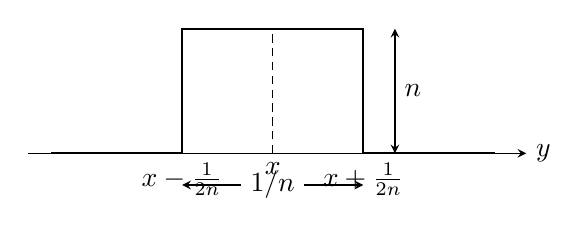
\begin{tikzpicture}[x=1.15cm,y=0.62cm,>=stealth]
  \draw[->] (-2.7,0) -- (2.8,0) node[right] {$y$};
  \draw[thick] (-2.45,0) -- (-1,0) -- (-1,2.55)
    -- (1,2.55) -- (1,0) -- (2.45,0);
  \draw[densely dashed] (0,0) -- (0,2.55);
  \draw[<->] (-1,-0.65) -- (1,-0.65)
    node[midway,fill=white] {$1/n$};
  \draw[<->] (1.35,0) -- (1.35,2.55)
    node[midway,right] {$n$};
  \node[below] at (-1,0) {$x-\frac1{2n}$};
  \node[below] at (0,0) {$x$};
  \node[below] at (1,0) {$x+\frac1{2n}$};
\end{tikzpicture}

{\small A narrower box is also taller, so its area remains one.}
\end{center}

If $f$ varies little across the box, then
\[
 \int_{-\infty}^{\infty}\psi_{x,n}(y)f(y)\dd y
 \approx f(x).
\]
The box approximately extracts the coefficient at $x$.

\begin{example}[Extracting a local value]
Let $f(y)=y^2$ and let the box have width $h$.

Its average is
\[
 \frac1h\int_{x-h/2}^{x+h/2}y^2\dd y
 =x^2+\frac{h^2}{12}.
\]
As $h\to0$, this tends to $x^2=f(x)$.
\end{example}

\section{The delta direction}

The idealised coordinate direction at $x$ is written $\delta_x$.

\begin{definition}[Delta direction at $x$: motivational form]
The symbol $\delta_x(y)$ is characterised heuristically by
\[
 \boxed{\int_{-\infty}^{\infty}
 \delta_x(y)f(y)\dd y=f(x).}
\]
It plays the role of the basis vector for the direction labelled by $x$.
\end{definition}

The narrow boxes motivate the notation
\[
 \psi_{x,n}(y)\longrightarrow\delta_x(y).
\]
No precise meaning of this limit is required here.

Just as $e_i$ extracts $v_i$, the delta direction extracts $f_x$:
\[
 \ip{e_i}{v}=v_i,
 \qquad
 \ip{\delta_x}{f}=f(x).
\]

The corresponding expansions are
\[
 v=\sum_i v_i e_i,
\]
and, heuristically,
\[
 \boxed{f(y)=\int_{-\infty}^{\infty}f(x)\delta_x(y)\dd x.}
\]

\subsection*{Moving the direction centred at zero}

First define the direction at the origin:
\[
 \delta_0(y)=\delta(y).
\]

Translate it from $0$ to $x$:
\[
 \boxed{\delta_x(y)=\delta_0(y-x).}
\]

The usual delta notation therefore gives
\[
 \delta_x(y)=\delta(y-x).
\]
Since the delta is symmetric,
\[
 \boxed{\delta_x(y)=\delta(y-x)=\delta(x-y).}
\]

This explains why an identity kernel is written
\[
 I(x,y)=\delta(x-y).
\]
Indeed,
\[
 (If)(x)=\int\delta(x-y)f(y)\dd y=f(x).
\]

\begin{caution}
The delta direction is not an ordinary $L^2$ function.

The unit-area boxes also satisfy
\[
 \norm{\psi_{x,n}}_2=\sqrt n.
\]
Their norms grow as they become narrower.  The delta notation is therefore
a coordinate picture, not an orthonormal basis inside $L^2$.
\end{caution}

A genuine orthonormal box approximation is obtained by dividing the line
into disjoint cells $I_j$ of width $h$ and setting
\[
 \phi_{j,h}(y)=\frac1{\sqrt h}\one_{I_j}(y).
\]
Then
\[
 \ip{\phi_{j,h}}{\phi_{k,h}}=\delta_{jk}.
\]
The coordinate is
\[
 c_j=\ip{\phi_{j,h}}{f}
 =\frac1{\sqrt h}\int_{I_j}f(y)\dd y.
\]
The reconstructed term is
\[
 c_j\phi_{j,h}(y)
 =\left(\frac1h\int_{I_j}f(s)\dd s\right)\one_{I_j}(y).
\]
Thus each cell is replaced by its average value.

\section{Why choose a Fourier basis?}

The position directions describe where a function is located.

For differentiation, oscillating directions are more useful:
\[
 \e^{\mathrm i nx}.
\]
Differentiation does not change their shape:
\[
 \frac{\dd}{\dd x}\e^{\mathrm i nx}
 =\mathrm i n\,\e^{\mathrm i nx}.
\]

This is the function-space analogue of choosing eigenvectors of a matrix.

In an eigenvector basis,
\[
 A\left(\sum_i c_iq_i\right)
 =\sum_i\lambda_i c_iq_i.
\]
In a Fourier basis, a differential operator will likewise multiply each
coefficient.

\section{The Fourier basis on $L^2(-\pi,\pi)$}

Complex notation combines sine and cosine into one expression.

Use the inner product
\[
 \ip{g}{f}
 =\int_{-\pi}^{\pi}\overline{g(x)}f(x)\dd x.
\]

\begin{definition}[Normalised complex Fourier functions]
For $n\in\Z$, define
\[
 \boxed{\phi_n(x)=\frac1{\sqrt{2\pi}}\e^{\mathrm i nx}.}
\]
\end{definition}

The factor $1/\sqrt{2\pi}$ makes every basis function have norm one:
\[
 \norm{\phi_n}_2^2
 =\frac1{2\pi}\int_{-\pi}^{\pi}1\dd x
 =1.
\]

\subsection*{Orthogonality}

For $m,n\in\Z$,
\[
 \begin{aligned}
 \ip{\phi_m}{\phi_n}
 &=\frac1{2\pi}\int_{-\pi}^{\pi}
   \e^{\mathrm i(n-m)x}\dd x.
 \end{aligned}
\]

If $m=n$, the integrand is $1$, so
\[
 \ip{\phi_n}{\phi_n}=1.
\]

If $m\ne n$, then
\[
 \begin{aligned}
 \ip{\phi_m}{\phi_n}
 &=\frac1{2\pi}
 \left[
 \frac{\e^{\mathrm i(n-m)x}}{\mathrm i(n-m)}
 \right]_{-\pi}^{\pi}\\
 &=0.
 \end{aligned}
\]
Hence
\[
 \boxed{\ip{\phi_m}{\phi_n}=\delta_{mn}.}
\]

\begin{proposition}[Fourier coordinates]
The coordinate of $f$ in the direction $\phi_n$ is
\[
 \boxed{
 c_n=\ip{\phi_n}{f}
 =\frac1{\sqrt{2\pi}}\int_{-\pi}^{\pi}
 f(x)\e^{-\mathrm i nx}\dd x.}
\]
The coordinate expansion is
\[
 \boxed{f(x)=\sum_{n\in\Z}c_n\phi_n(x)}
\]
in the $L^2$ sense.
\end{proposition}

\begin{bridge}
A Fourier coefficient is not a new kind of object.

It is simply a coordinate in the Fourier basis:
\[
 \boxed{\text{Fourier coefficient}
 =\text{coordinate in the Fourier basis}.}
\]
The phrase \emph{Fourier series} means the corresponding basis expansion.
\end{bridge}

A second common convention uses
\[
 \widehat f_n
 =\frac1{2\pi}\int_{-\pi}^{\pi}
 f(x)\e^{-\mathrm i nx}\dd x.
\]
Then
\[
 f(x)=\sum_{n\in\Z}\widehat f_n\e^{\mathrm i nx}.
\]
The two conventions differ only by normalisation:
\[
 c_n=\sqrt{2\pi}\,\widehat f_n.
\]

\subsection*{The real sine and cosine basis}

Euler's formula gives
\[
 \e^{\mathrm i nx}=\cos(nx)+\mathrm i\sin(nx).
\]
Also,
\[
 \cos(nx)
 =\frac{\e^{\mathrm i nx}+\e^{-\mathrm i nx}}2,
\]
\[
 \sin(nx)
 =\frac{\e^{\mathrm i nx}-\e^{-\mathrm i nx}}
 {2\mathrm i}.
\]

Thus the real and complex descriptions contain the same oscillations.

A real orthonormal basis is
\[
 \boxed{
 \frac1{\sqrt{2\pi}},
 \qquad
 \frac{\cos(nx)}{\sqrt\pi},
 \qquad
 \frac{\sin(nx)}{\sqrt\pi},
 \quad n=1,2,\ldots .}
\]

\section{Changing the interval to $(-L,L)$}

The interval now has length $2L$.

To fit exactly across this interval, the frequencies become
\[
 k_n=\frac{n\pi}{L}.
\]

\begin{definition}[Fourier basis on $(-L,L)$]
For $n\in\Z$, define
\[
 \boxed{
 \phi_n^{(L)}(x)
 =\frac1{\sqrt{2L}}
 \e^{\mathrm i n\pi x/L}.}
\]
\end{definition}

The normalisation again gives unit norm:
\[
 \norm{\phi_n^{(L)}}_2^2
 =\frac1{2L}\int_{-L}^{L}1\dd x
 =1.
\]

Orthogonality follows from
\[
 \ip{\phi_m^{(L)}}{\phi_n^{(L)}}
 =\frac1{2L}\int_{-L}^{L}
 \e^{\mathrm i(n-m)\pi x/L}\dd x
 =\delta_{mn}.
\]

The real orthonormal basis is
\[
 \boxed{
 \frac1{\sqrt{2L}},
 \qquad
 \frac{\cos(n\pi x/L)}{\sqrt L},
 \qquad
 \frac{\sin(n\pi x/L)}{\sqrt L},
 \quad n=1,2,\ldots .}
\]

\begin{bridge}
Nothing essential has changed.

On $(-\pi,\pi)$:
\[
 n\quad\text{is the wave number}.
\]

On $(-L,L)$:
\[
 \frac{n\pi}{L}\quad\text{is the wave number}.
\]

The interval length changes the allowed frequencies and the normalising
constant.
\end{bridge}

\section{Real Fourier series and three examples}

For a real function on $(-L,L)$, the conventional form is
\[
 f(x)\sim
 \frac{a_0}{2}
 +\sum_{n=1}^{\infty}
 \left[
 a_n\cos\!\left(\frac{n\pi x}{L}\right)
 +b_n\sin\!\left(\frac{n\pi x}{L}\right)
 \right],
\]
where
\[
 a_n=\frac1L\int_{-L}^{L}
 f(x)\cos\!\left(\frac{n\pi x}{L}\right)\dd x,
\]
\[
 b_n=\frac1L\int_{-L}^{L}
 f(x)\sin\!\left(\frac{n\pi x}{L}\right)\dd x.
\]

These $a_n$ and $b_n$ are again coordinates, with a conventional
normalisation.

Even functions have only cosine terms.

Odd functions have only sine terms.

\subsection*{What happens at a jump?}

Suppose $f$ has one-sided limits at $x$:
\[
 f(x^-),
 \qquad
 f(x^+).
\]
For a piecewise smooth function, its Fourier series converges there to
\[
 \boxed{\frac{f(x^-)+f(x^+)}2.}
\]

At a continuous point this is simply $f(x)$.

At a jump it is the midpoint between the two limiting values.

This does not conflict with $L^2$ equality: changing a function at one point
does not change its $L^2$ vector.

\begin{example}[The function $x^2$ on $(-\pi,\pi)$]
The function is even, so $b_n=0$.

Its coefficients are
\[
 a_0=\frac1\pi\int_{-\pi}^{\pi}x^2\dd x
 =\frac{2\pi^2}{3},
\]
\[
 a_n=\frac1\pi\int_{-\pi}^{\pi}x^2\cos(nx)\dd x
 =\frac{4(-1)^n}{n^2}.
\]
Therefore
\[
 \boxed{
 x^2=\frac{\pi^2}{3}
 +4\sum_{n=1}^{\infty}
 \frac{(-1)^n}{n^2}\cos(nx).}
\]
At $x=\pi$, this gives
\[
 \pi^2=\frac{\pi^2}{3}
 +4\sum_{n=1}^{\infty}\frac1{n^2}.
\]
Hence
\[
 \sum_{n=1}^{\infty}\frac1{n^2}
 =\frac{\pi^2}{6}.
\]
\end{example}

\begin{example}[A step function]
On $(-\pi,\pi)$, define
\[
 s(x)=
 \begin{cases}
 -1,&-\pi<x<0,\\
 1,&0<x<\pi.
 \end{cases}
\]
The function is odd, so only sine coordinates occur:
\[
 \boxed{
 s(x)\sim\frac4\pi
 \sum_{r=0}^{\infty}
 \frac{\sin((2r+1)x)}{2r+1}.}
\]

At $x=0$,
\[
 s(0^- )=-1,
 \qquad
 s(0^+)=1.
\]
The Fourier series therefore takes the midpoint value
\[
 \frac{-1+1}{2}=0.
\]
Every sine term is also zero at $x=0$.

At $x=\pi$, the periodic extension jumps from $1$ back to $-1$.
The series again converges to $0$.
\end{example}

\begin{example}[The tent function $1-|x|$ on $(-1,1)$]
Let
\[
 f(x)=1-|x|.
\]
This function is even and has period $2$ after periodic extension.

Its Fourier series is
\[
 \boxed{
 1-|x|
 =\frac12+\frac4{\pi^2}
 \sum_{r=0}^{\infty}
 \frac{\cos((2r+1)\pi x)}{(2r+1)^2}.}
\]
Only odd cosine modes occur.

At $x=0$,
\[
 1=\frac12+\frac4{\pi^2}
 \sum_{r=0}^{\infty}\frac1{(2r+1)^2}.
\]
At $x=1$,
\[
 0=\frac12-\frac4{\pi^2}
 \sum_{r=0}^{\infty}\frac1{(2r+1)^2}.
\]
Both give
\[
 \sum_{r=0}^{\infty}\frac1{(2r+1)^2}
 =\frac{\pi^2}{8}.
\]
\end{example}

\section{Parseval's identity}

For an orthonormal basis in $\R^N$,
\[
 \norm{v}^2=\sum_i|c_i|^2.
\]
The length of the vector equals the length of its coordinate list.

The same statement holds for Fourier coordinates.

\begin{theorem}[Parseval on $(-\pi,\pi)$]
If
\[
 f=\sum_{n\in\Z}c_n\phi_n,
\]
then
\[
 \boxed{
 \int_{-\pi}^{\pi}|f(x)|^2\dd x
 =\sum_{n\in\Z}|c_n|^2.}
\]
\end{theorem}

For the conventional real coefficients on $(-L,L)$,
\[
 \boxed{
 \frac1L\int_{-L}^{L}|f(x)|^2\dd x
 =\frac{a_0^2}{2}
 +\sum_{n=1}^{\infty}(a_n^2+b_n^2).}
\]

\begin{bridge}
Parseval says that changing to Fourier coordinates does not change length.

It is the function-space version of
\[
 P^{-1}=P^T
\]
for an orthogonal change of basis in $\R^N$.
\end{bridge}

\begin{example}[Parseval for the step function]
For the step function, $|s(x)|^2=1$ almost everywhere.  Hence
\[
 \frac1\pi\int_{-\pi}^{\pi}|s(x)|^2\dd x=2.
\]
Its non-zero sine coefficients are
\[
 b_{2r+1}=\frac4{\pi(2r+1)}.
\]
Parseval gives
\[
 2=\frac{16}{\pi^2}
 \sum_{r=0}^{\infty}\frac1{(2r+1)^2},
\]
again yielding
\[
 \sum_{r=0}^{\infty}\frac1{(2r+1)^2}
 =\frac{\pi^2}{8}.
\]
\end{example}

\section{Differential operators multiply Fourier coordinates}

On $(-L,L)$,
\[
 \phi_n^{(L)}(x)
 =\frac1{\sqrt{2L}}\e^{\mathrm i n\pi x/L}.
\]
Therefore
\[
 \frac{\dd}{\dd x}\phi_n^{(L)}
 =\frac{\mathrm i n\pi}{L}\phi_n^{(L)},
\]
and
\[
 -\frac{\dd^2}{\dd x^2}\phi_n^{(L)}
 =\left(\frac{n\pi}{L}\right)^2\phi_n^{(L)}.
\]

If
\[
 f=\sum_{n\in\Z}c_n\phi_n^{(L)},
\]
then, formally,
\[
 \boxed{
 f'
 =\sum_{n\in\Z}
 \left(\frac{\mathrm i n\pi}{L}\right)
 c_n\phi_n^{(L)},}
\]
and
\[
 \boxed{
 -f''
 =\sum_{n\in\Z}
 \left(\frac{n\pi}{L}\right)^2
 c_n\phi_n^{(L)}.}
\]

Thus differentiation acts directly on the coordinates:
\[
 c_n\longmapsto
 \frac{\mathrm i n\pi}{L}c_n,
\]
\[
 c_n\longmapsto
 \left(\frac{n\pi}{L}\right)^2c_n.
\]

\begin{bridge}
Compare the three calculations:
\[
 \begin{aligned}
 A q_i&=\lambda_iq_i,
 &c_i&\longmapsto\lambda_i c_i,\\
 D\phi_n^{(L)}
 &=\frac{\mathrm i n\pi}{L}\phi_n^{(L)},
 &c_n&\longmapsto\frac{\mathrm i n\pi}{L}c_n.
 \end{aligned}
\]
The operator is complicated in the original coordinates but simple in its
eigenbasis.
\end{bridge}

\begin{example}[Differentiate one Fourier mode]
On $(-\pi,\pi)$,
\[
 f(x)=\cos(3x)
 =\frac12\e^{3\mathrm i x}
 +\frac12\e^{-3\mathrm i x}.
\]
Differentiation multiplies the two coordinates by $3\mathrm i$ and
$-3\mathrm i$:
\[
 f'(x)
 =\frac{3\mathrm i}{2}\e^{3\mathrm i x}
 -\frac{3\mathrm i}{2}\e^{-3\mathrm i x}.
\]
Therefore
\[
 f'(x)=-3\sin(3x).
\]
\end{example}

\section{The periodic heat equation}

Consider the heat equation on $(-L,L)$:
\[
 \frac{\partial u}{\partial t}
 =\kappa\frac{\partial^2u}{\partial x^2},
 \qquad
 u(x,0)=f(x),
\]
with periodic boundary conditions.

At each time $t$, expand the function-vector:
\[
 \boxed{
 u(x,t)=\sum_{n\in\Z}c_n(t)\phi_n^{(L)}(x).}
\]
This is exactly the form
\[
 v(t)=\sum_i c_i(t)e_i
\]
from finite-dimensional linear algebra.

The coefficients are now time-dependent.

Differentiate with respect to time:
\[
 u_t
 =\sum_{n\in\Z}c_n'(t)\phi_n^{(L)}.
\]
Differentiate twice with respect to position:
\[
 u_{xx}
 =-\sum_{n\in\Z}
 \left(\frac{n\pi}{L}\right)^2
 c_n(t)\phi_n^{(L)}.
\]

Equality of the two function-vectors means equality of every coordinate:
\[
 c_n'(t)
 =-\kappa\left(\frac{n\pi}{L}\right)^2c_n(t).
\]
The partial differential equation has become one scalar ordinary
differential equation for each $n$.

\begin{theorem}[Periodic heat flow]
Let
\[
 c_n(0)=\ip{\phi_n^{(L)}}{f}.
\]
Then
\[
 \boxed{
 c_n(t)
 =\exp\!\left[
 -\kappa\left(\frac{n\pi}{L}\right)^2t
 \right]c_n(0).}
\]
Hence
\[
 \boxed{
 u(x,t)=\sum_{n\in\Z}
 \exp\!\left[
 -\kappa\left(\frac{n\pi}{L}\right)^2t
 \right]
 c_n(0)\phi_n^{(L)}(x).}
\]
\end{theorem}

The $n=0$ coordinate is unchanged.

Coordinates with large $|n|$ decay quickly.

Large $|n|$ corresponds to rapid oscillation, so heat flow removes fine
detail first.

\begin{example}[Two temperature modes]
On $(-\pi,\pi)$, suppose
\[
 u(x,0)=3+2\cos x+\frac12\cos(4x).
\]
Then
\[
 \boxed{
 u(x,t)=3+2\e^{-\kappa t}\cos x
 +\frac12\e^{-16\kappa t}\cos(4x).}
\]
The fourth mode decays much faster than the first.

The constant coordinate $3$ is the mean temperature and remains fixed.
\end{example}

\begin{bridge}
Let
\[
 A=-\frac{\partial^2}{\partial x^2}.
\]
Then the heat equation is
\[
 u_t=-\kappa Au.
\]

This mirrors the finite-dimensional equation
\[
 v'(t)=-\kappa Av(t).
\]
In an eigenbasis of $A$, each coordinate evolves independently:
\[
 c_n'(t)=-\kappa\lambda_n c_n(t).
\]
\end{bridge}

\section{From a Fourier series to a Fourier transform}

Now enlarge the interval:
\[
 (-L,L)\longrightarrow\R.
\]

On $(-L,L)$, the wave numbers are
\[
 k_n=\frac{n\pi}{L}.
\]
The spacing between neighbouring wave numbers is
\[
 \Delta k=\frac{\pi}{L}.
\]
As $L\to\infty$,
\[
 \Delta k\to0.
\]
The discrete frequency label $n$ is replaced by a continuous label $k$.

For a function concentrated well inside $(-L,L)$,
\[
 c_n
 =\frac1{\sqrt{2L}}\int_{-L}^{L}
 f(x)\e^{-\mathrm i k_nx}\dd x.
\]
If
\[
 \widehat f(k)
 =\frac1{\sqrt{2\pi}}\int_{-\infty}^{\infty}
 f(x)\e^{-\mathrm i kx}\dd x,
\]
then heuristically
\[
 c_n\approx\sqrt{\Delta k}\,\widehat f(k_n).
\]

Also,
\[
 \phi_n^{(L)}(x)
 =\sqrt{\frac{\Delta k}{2\pi}}\,
 \e^{\mathrm i k_nx}.
\]
Therefore
\[
 \sum_n c_n\phi_n^{(L)}(x)
 \approx
 \sum_n
 \frac{\Delta k}{\sqrt{2\pi}}
 \widehat f(k_n)\e^{\mathrm i k_nx}.
\]
As the spacing tends to zero, the sum suggests the integral
\[
 \frac1{\sqrt{2\pi}}\int_{-\infty}^{\infty}
 \widehat f(k)\e^{\mathrm i kx}\dd k.
\]

\begin{caution}
This passage from $L^2(-L,L)$ to $L^2(\R)$ is motivational.

It correctly predicts the formulas, but a rigorous proof requires care
about limits, convergence and the fact that plane waves are not in
$L^2(\R)$.
\end{caution}

\section{Fourier coordinates on $L^2(\R)$}

The position picture uses the continuous family $\delta_x$.

The frequency picture uses the continuous family
\[
 \phi_k(x)=\frac1{\sqrt{2\pi}}\e^{\mathrm i kx},
 \qquad k\in\R.
\]

These plane waves are not ordinary $L^2(\R)$ vectors.  They are generalised
basis functions.

Heuristically,
\[
 \ip{\phi_k}{\phi_q}=\delta(k-q).
\]

\begin{definition}[Fourier transform]
The Fourier coefficient in the direction $\phi_k$ is
\[
 \boxed{
 \widehat f(k)
 =\ip{\phi_k}{f}
 =\frac1{\sqrt{2\pi}}\int_{-\infty}^{\infty}
 f(x)\e^{-\mathrm i kx}\dd x.}
\]
The function $k\mapsto\widehat f(k)$ is called the Fourier transform.
\end{definition}

\begin{bridge}
The terminology changes, but the object does not.

For a discrete basis:
\[
 c_n=\ip{\phi_n}{f}
 \quad\text{is a Fourier coefficient}.
\]

For a continuous basis:
\[
 \widehat f(k)=\ip{\phi_k}{f}
 \quad\text{is a Fourier coefficient}.
\]

The Fourier transform is simply the continuous list of Fourier
coefficients.
\end{bridge}

\begin{definition}[Inverse Fourier transform]
The continuous basis expansion is
\[
 \boxed{
 f(x)=\frac1{\sqrt{2\pi}}
 \int_{-\infty}^{\infty}
 \widehat f(k)\e^{\mathrm i kx}\dd k.}
\]
Equivalently,
\[
 f=\int_{-\infty}^{\infty}\widehat f(k)\phi_k\dd k.
\]
\end{definition}

Compare:
\[
 v=\sum_i c_i e_i,
\]
\[
 f=\sum_n c_n\phi_n,
\]
\[
 f=\int\widehat f(k)\phi_k\dd k.
\]
Only the index set has changed.

The continuous Parseval identity is
\[
 \boxed{
 \int_{-\infty}^{\infty}|f(x)|^2\dd x
 =\int_{-\infty}^{\infty}|\widehat f(k)|^2\dd k.}
\]
Thus the Fourier transform preserves the length of the vector.

\section{Differential operators in Fourier coordinates}

The plane waves are eigenfunctions of differentiation:
\[
 \frac{\dd}{\dd x}\phi_k=\mathrm i k\phi_k,
\]
\[
 -\frac{\dd^2}{\dd x^2}\phi_k=k^2\phi_k.
\]

Therefore differentiation multiplies Fourier coefficients.

\begin{proposition}[Fourier multipliers]
When boundary terms vanish,
\[
 \boxed{\widehat{f'}(k)=\mathrm i k\,\widehat f(k),}
\]
and
\[
 \boxed{\widehat{-f''}(k)=k^2\widehat f(k).}
\]
More generally,
\[
 \widehat{p(D)f}(k)
 =p(\mathrm i k)\widehat f(k),
 \qquad
 D=\frac{\dd}{\dd x}.
\]
\end{proposition}

The finite and continuous calculations are identical:
\[
 c_i\longmapsto\lambda_i c_i,
\]
\[
 c_n\longmapsto\lambda_n c_n,
\]
\[
 \widehat f(k)\longmapsto\lambda(k)\widehat f(k).
\]

\section{The Gaussian transforms to a Gaussian}

\begin{proposition}[Gaussian Fourier transform]
For $a>0$,
\[
 f(x)=\e^{-ax^2}
\]
has Fourier transform
\[
 \boxed{
 \widehat f(k)
 =\frac1{\sqrt{2a}}\e^{-k^2/(4a)}.}
\]
\end{proposition}

\begin{proof}
The standard Gaussian integral gives
\[
 \int_{-\infty}^{\infty}
 \e^{-ax^2-\mathrm i kx}\dd x
 =\sqrt{\frac\pi a}\,
 \e^{-k^2/(4a)}.
\]
Multiply by $1/\sqrt{2\pi}$.
\end{proof}

For the unit-area Gaussian
\[
 g_\sigma(x)
 =\frac1{\sqrt{2\pi\sigma^2}}
 \exp\!\left(-\frac{x^2}{2\sigma^2}\right),
\]
one obtains
\[
 \boxed{
 \widehat g_\sigma(k)
 =\frac1{\sqrt{2\pi}}
 \e^{-\sigma^2k^2/2}.}
\]

A narrow Gaussian in position has a broad Fourier transform.

A broad Gaussian in position has a narrow Fourier transform.

\section{The heat equation on the real line}

Consider
\[
 u_t=\kappa u_{xx},
 \qquad
 x\in\R,
 \qquad
 u(x,0)=f(x).
\]

For each time $t$, take the Fourier coefficient in the $k$ direction:
\[
 \widehat u(k,t)
 =\frac1{\sqrt{2\pi}}\int_{\R}
 u(x,t)\e^{-\mathrm i kx}\dd x.
\]
The transform of $u_{xx}$ is
\[
 -k^2\widehat u(k,t).
\]
Hence every Fourier coordinate satisfies
\[
 \frac{\partial\widehat u}{\partial t}(k,t)
 =-\kappa k^2\widehat u(k,t).
\]

This is the continuous version of
\[
 c_n'(t)=-\kappa\lambda_n c_n(t).
\]

\begin{theorem}[Heat flow on $\R$]
The Fourier coefficients evolve by
\[
 \boxed{
 \widehat u(k,t)
 =\e^{-\kappa k^2t}\widehat f(k).}
\]
After inverse transformation,
\[
 \boxed{u(x,t)=(G_t*f)(x),}
\]
where
\[
 \boxed{
 G_t(x)=\frac1{\sqrt{4\pi\kappa t}}
 \exp\!\left(-\frac{x^2}{4\kappa t}\right).}
\]
\end{theorem}

The Gaussian calculation shows that
\[
 \widehat G_t(k)
 =\frac1{\sqrt{2\pi}}\e^{-\kappa k^2t}.
\]
Thus convolution with $G_t$ produces exactly the required multiplier.

\begin{bridge}
The kernel $G_t$ has total area one:
\[
 \int_{\R}G_t(x)\dd x=1.
\]
It is a smooth averaging box.

The value $u(x,t)$ is a weighted average of the initial temperature near
$x$.  The averaging width grows like
\[
 \sqrt{\kappa t}.
\]

If the initial temperature is the ideal position direction $\delta_0$, then
\[
 u(x,t)=G_t(x).
\]
A point of heat spreads into a Gaussian.
\end{bridge}

\begin{example}[A Gaussian spreads]
If
\[
 f(x)=g_\sigma(x),
\]
then
\[
 \boxed{
 u(x,t)
 =g_{\sqrt{\sigma^2+2\kappa t}}(x).}
\]
The total heat remains one.

The variance changes by
\[
 \sigma^2\longmapsto\sigma^2+2\kappa t.
\]
\end{example}

\section{The infinite square well}

Quantum wavefunctions are complex function-vectors on $(0,L)$:
\[
 \ip{\phi}{\psi}
 =\int_0^L\overline{\phi(x)}\psi(x)\dd x.
\]

\begin{definition}[Infinite potential well]
The potential is zero for $0<x<L$ and infinite outside.

The wavefunction obeys
\[
 \psi(0,t)=\psi(L,t)=0.
\]
Inside the well,
\[
 \boxed{
 H=-\frac{\hbar^2}{2m}\frac{\dd^2}{\dd x^2}.}
\]
\end{definition}

First find a basis adapted to $H$:
\[
 H\phi=E\phi.
\]
Thus
\[
 -\frac{\hbar^2}{2m}\phi''=E\phi.
\]
Write
\[
 k^2=\frac{2mE}{\hbar^2}.
\]
Then
\[
 \phi(x)=A\sin(kx)+B\cos(kx).
\]

The boundary condition $\phi(0)=0$ gives
\[
 B=0.
\]
The condition $\phi(L)=0$ gives
\[
 \sin(kL)=0.
\]
Therefore
\[
 k=\frac{n\pi}{L},
 \qquad n=1,2,\ldots .
\]

\begin{theorem}[Energy eigenbasis]
The normalised eigenfunctions are
\[
 \boxed{
 \phi_n(x)
 =\sqrt{\frac2L}
 \sin\!\left(\frac{n\pi x}{L}\right).}
\]
Their energies are
\[
 \boxed{
 E_n=\frac{\hbar^2\pi^2n^2}{2mL^2}.}
\]
Moreover,
\[
 H\phi_n=E_n\phi_n.
\]
\end{theorem}

Expand the initial state in the energy basis:
\[
 \psi(x,0)
 =\sum_{n=1}^{\infty}c_n(0)\phi_n(x),
\]
where
\[
 c_n(0)=\ip{\phi_n}{\psi(\,\cdot\,,0)}.
\]

At time $t$, allow the coordinates to move:
\[
 \psi(x,t)
 =\sum_{n=1}^{\infty}c_n(t)\phi_n(x).
\]
Substitute this into
\[
 \mathrm i\hbar\psi_t=H\psi.
\]

The left-hand side is
\[
 \mathrm i\hbar
 \sum_n c_n'(t)\phi_n.
\]
The right-hand side is
\[
 \sum_n E_nc_n(t)\phi_n.
\]
Equality of coordinates gives
\[
 \mathrm i\hbar c_n'(t)=E_nc_n(t).
\]

\begin{theorem}[Time evolution in the well]
Each energy coordinate evolves independently:
\[
 \boxed{
 c_n(t)
 =\e^{-\mathrm iE_nt/\hbar}c_n(0).}
\]
Therefore
\[
 \boxed{
 \psi(x,t)
 =\sum_{n=1}^{\infty}
 c_n(0)\e^{-\mathrm iE_nt/\hbar}\phi_n(x).}
\]
\end{theorem}

The Hamiltonian multiplies the $n$th coordinate by $E_n$.

Time evolution multiplies it by a phase:
\[
 \e^{-\mathrm iE_nt/\hbar}.
\]
Its magnitude is one, so
\[
 |c_n(t)|=|c_n(0)|.
\]

\begin{example}[Two energy levels]
Suppose
\[
 \psi(x,0)
 =\frac1{\sqrt2}
 \bigl(\phi_1(x)+\phi_2(x)\bigr).
\]
Then
\[
 \begin{aligned}
 \psi(x,t)
 =\frac1{\sqrt2}\bigl(
 &\e^{-\mathrm iE_1t/\hbar}\phi_1(x)\\
 &+\e^{-\mathrm iE_2t/\hbar}\phi_2(x)
 \bigr).
 \end{aligned}
\]
The two coefficient magnitudes remain $1/\sqrt2$.

Only their phases change.

The relative phase is
\[
 \frac{(E_2-E_1)t}{\hbar}.
\]
\end{example}

\section{Heat flow and quantum motion compared}

Both equations become scalar equations in an eigenbasis.

\begin{center}
\renewcommand{\arraystretch}{1.45}
\begin{tabularx}{\textwidth}{@{}>{\bfseries}p{.23\textwidth}XX@{}}
\toprule
 & Heat equation & Schr\"odinger equation\\
\midrule
Equation
& $u_t=-Au$
& $\mathrm i\hbar\psi_t=H\psi$\\
Coordinate
& $c_n(t)$
& $c_n(t)$\\
Evolution
& $\e^{-\lambda_nt}c_n(0)$
& $\e^{-\mathrm iE_nt/\hbar}c_n(0)$\\
Effect
& Magnitudes decay
& Magnitudes remain fixed\\
Meaning
& Smoothing
& Phase rotation\\
\bottomrule
\end{tabularx}
\end{center}

\begin{summarybox}
\centering
\small
\renewcommand{\arraystretch}{1.45}
\begin{tabularx}{\linewidth}{@{}>{\raggedright\arraybackslash}X
  >{\centering\arraybackslash}p{.20\linewidth}
  >{\centering\arraybackslash}p{.29\linewidth}@{}}
\textbf{Basis direction} & \textbf{Coordinate} & \textbf{Multiplier}\\
\midrule
$q_i$ & $c_i$ & $\lambda_i$\\
$\e^{\mathrm i n\pi x/L}$ & $c_n$ &
 $\mathrm i n\pi/L$ or $(n\pi/L)^2$\\
$\e^{\mathrm i kx}$ & $\widehat f(k)$ &
 $\mathrm i k$ or $k^2$\\
$\sin(n\pi x/L)$ & $c_n$ & $E_n$
\end{tabularx}
\end{summarybox}

The repeated method is:
\[
 \boxed{
 \begin{gathered}
 \text{choose a basis adapted to the operator},\\
 \text{take coordinates},\\
 \text{multiply each coordinate},\\
 \text{reconstruct the vector}.
 \end{gathered}}
\]

% =============================================================================
\part{Synthesis}
\chapter{The Three-Part Dictionary}

\section*{One idea, three index sets}
\addcontentsline{toc}{section}{One idea, three index sets}

The central message can be compressed into two lines:
\[
 \boxed{\text{finite indices}
 \ \longrightarrow\ \text{countable indices}
 \ \longrightarrow\ \text{continuous indices}},
\]
\[
 \boxed{\sum_i\ \longrightarrow\ \sum_n\
 \longrightarrow\ \sum_x\;(\text{heuristic})
 \rightsquigarrow\ \int\dd x}.
\]
The table follows the common section numbering.

\clearpage
\newgeometry{top=13mm,bottom=13mm,left=12mm,right=12mm,headheight=14pt}
\begin{landscape}
\small
\renewcommand{\arraystretch}{1.40}
\setlength{\tabcolsep}{4.5pt}
\begin{longtable}{>{\raggedright\arraybackslash\bfseries}p{0.16\linewidth}
                  >{\raggedright\arraybackslash}p{0.25\linewidth}
                  >{\raggedright\arraybackslash}p{0.25\linewidth}
                  >{\raggedright\arraybackslash}p{0.25\linewidth}}
\caption{Parallel dictionary for finite vectors, sequences and functions}
\label{tab:dictionary}\\
\toprule
Concept & Part I: $\R^N$ & Part II: $\ell^2$ & Part III: $L^2(I)$\\
\midrule
\endfirsthead
\multicolumn{4}{l}{\small\sffamily Table \thetable\ continued}\\
\toprule
Concept & Part I: $\R^N$ & Part II: $\ell^2$ & Part III: $L^2(I)$\\
\midrule
\endhead
\midrule
\multicolumn{4}{r}{\small Continued on next page}\\
\endfoot
\bottomrule
\endlastfoot

Underlying vector & $v=(v_1,\ldots,v_N)$ &
$a=(a_1,a_2,\ldots)$ &
$f=(f_x)_{x\in I}$ initially; then $f(x)$\\

Index set & $i=1,\ldots,N$ & $n\in\N$ & $x\in I\subseteq\R$\\

Natural space & $\R^N$ &
$\ell^2=\{a:\sum_n a_n^2<\infty\}$ &
$L^2(I)=\{f:\int_I|f|^2<\infty\}$ modulo equality almost everywhere\\

Coordinate sum & $\sum_{i=1}^{N}$ & $\sum_{n=1}^{\infty}$ &
$\sum_x$ only as motivation; rigorously $\int_I\dd x$\\

Linear combination & $\sum_{j=1}^{k}\alpha_jv_j$ &
Finite algebraic combinations; limits add infinite expansions &
Finite algebraic combinations; limits produce function expansions\\

Standard or useful basis & Standard vectors $e_i$ &
Standard sequences $e_n$ &
Problem-adapted basis functions, e.g. $\sqrt{2/\pi}\sin(nx)$ on $(0,\pi)$\\

Basis meaning & Finite algebraic basis &
Complete orthonormal system with norm-convergent series &
Complete orthonormal system with $L^2$-convergent series\\

Decomposition & $v=\sum_i v_ie_i$ &
$a=\sum_n a_ne_n$ in $\ell^2$ &
$f=\sum_n c_n\phi_n$ in $L^2$, $c_n=\ip{\phi_n}{f}$\\

New convergence issue & None: sums are finite &
Series and truncation tails must converge &
$L^2$ convergence need not imply pointwise convergence\\

Linear operator & $A:\R^N\to\R^N$ &
Bounded $A:\ell^2\to\ell^2$, or unbounded $A$ with a domain &
Multiplication, differentiation and integral operators; domains and boundary
conditions matter\\

Component action & $(Av)_i=\sum_jA_{ij}v_j$ &
$(Aa)_n=\sum_mA_{nm}a_m$ &
$(Af)_x=\sum_y(A_{xy}f_y)\rightsquigarrow
\int_IA(x,y)f(y)\dd y$\\

Matrix or kernel & Finite matrix $(A_{ij})$ &
Infinite matrix $(A_{nm})$ when its series defines an operator &
Kernel $A(x,y)$, a continuously indexed matrix\\

Inner product & $\ip{u}{v}=\sum_i u_iv_i$ &
$\ip{a}{b}=\sum_n a_nb_n$ &
$\sum_x(f_xg_x)\rightsquigarrow\ip{f}{g}=\int_If(x)g(x)\dd x$\\

$p$-norm & $\norm{v}_p=(\sum_i|v_i|^p)^{1/p}$ &
$\norm{a}_p=(\sum_n|a_n|^p)^{1/p}$ &
$\norm{f}_p=(\int_I|f|^p)^{1/p}$\\

Norm equivalence & All $p$-norms equivalent on fixed $\R^N$;
$C^{-1}\norm{v}_p\le\norm{v}_q\le C\norm{v}_p$ &
Fails: block-vector norm ratios grow without bound; $\ell^p$ spaces differ &
Fails: concentrating spikes have incompatible norm ratios; $L^p$ spaces differ\\

Normalisation & $\widehat v=v/\norm{v}_2$ &
$\widehat a=a/\norm{a}_2$ & $\widehat f=f/\norm{f}_2$\\

Orthogonality & $\sum_i u_iv_i=0$ & $\sum_na_nb_n=0$ &
$\int_If(x)g(x)\dd x=0$\\

Projection onto a unit basis element & $P_iv=\ip{e_i}{v}e_i$ &
$P_na=\ip{e_n}{a}e_n$ & $P_\phi f=\ip{\phi}{f}\phi$\\

Projection kernel & $P_i=e_ie_i^T$ &
$(P_n)_{jk}=\delta_{jn}\delta_{kn}$ &
$P_\phi(x,y)=\phi(x)\phi(y)$\\

Resolution of identity & $I=\sum_{i=1}^{N}P_i$ &
$I=\sum_{n=1}^{\infty}P_n$ strongly &
$I=\sum_nP_n$ in a complete basis; formally $I(x,y)=\delta(x-y)$\\

Parseval & $\norm{v}_2^2=\sum_i|\ip{e_i}{v}|^2$ &
$\norm{a}_2^2=\sum_n|\ip{e_n}{a}|^2$ &
$\norm{f}_2^2=\sum_n|\ip{\phi_n}{f}|^2$\\

Eigen-equation & $Av=\lambda v$ & $Aa=\lambda a$ & $Af=\lambda f$\\

Eigen-object & Eigenvector & Eigenvector (sequence) & Eigenfunction\\

Eigenspace and degeneracy & $E_\lambda=\Ker(A-\lambda I)$; finite dimension &
Eigenspace may have finite or infinite dimension &
Boundary conditions influence eigenspaces; symmetry can create degeneracy\\

Adjoint & $A^*=A^T$ in a real orthonormal basis &
$\ip{a}{Ab}=\ip{A^*a}{b}$; domains matter if unbounded &
$\ip{f}{Ag}=\ip{A^*f}{g}$; transpose the kernel or integrate by parts\\

Self-adjoint & Real symmetric matrix & $A=A^*$ with matching domains &
$A=A^*$ with boundary conditions included in the domain\\

Eigenvalue consequence & Self-adjoint eigenvalues are real & Same & Same\\

Eigenvector consequence & Distinct eigenvalues give orthogonal eigenvectors &
Same, when eigenvectors exist & Distinct eigenvalues give orthogonal eigenfunctions\\

Spectral theorem & Every self-adjoint operator has an orthonormal eigenbasis &
Compact self-adjoint operators have a discrete eigenbasis; general operators
may require spectral measures &
Compact symmetric kernels often have eigenfunction bases; multiplication and
differential operators may have continuous spectrum\\

Spectral decomposition & $A=\sum_\lambda\lambda P_\lambda$ &
$A=\sum_n\lambda_nP_n$ in the discrete case; generally
 $A=\int\lambda\dd P(\lambda)$ &
 Discrete eigenfunction sums or the spectral integral
 $A=\int\lambda\dd P(\lambda)$\\*

Characteristic new issue & Basis choice, but no analytical obstruction &
Convergence, completeness, boundedness and domains &
Integration, almost-everywhere equality, boundary conditions and continuous
spectrum\\
\end{longtable}
\end{landscape}
\restoregeometry

\section*{A final worked bridge: one-dimensional projection}
\addcontentsline{toc}{section}{A final worked bridge}

Choose a normalised direction in each setting:
\[
 e_i\in\R^N,
 \qquad e_n\in\ell^2,
 \qquad \phi\in L^2(I).
\]
Projection is always ``overlap times direction'':
\[
 \begin{aligned}
 P_iv
   &=\left(\sum_{j=1}^{N}(e_i)_jv_j\right)e_i,\\[1mm]
 P_na
   &=\left(\sum_{m=1}^{\infty}(e_n)_ma_m\right)e_n,\\[1mm]
 P_\phi f
   &=\left(\int_I\phi(y)f(y)\dd y\right)\phi.
 \end{aligned}
\]
In kernel notation the last line is
\[
 (P_\phi f)(x)=\int_I\underbrace{\phi(x)\phi(y)}_{P_\phi(x,y)}f(y)\dd y.
\]
Only the index set, and hence the summation rule, has changed.

\begin{summarybox}
\centering
\sffamily\bfseries\large
You have already seen the idea.  Only the index set has changed.
\end{summarybox}

\chapter*{Closing perspective}
\addcontentsline{toc}{chapter}{Closing perspective}

A function is a vector.  A Fourier coefficient is a coordinate.  An integral
kernel is a matrix.  A modal expansion is a spectral decomposition.

In infinite dimensions, ask:
\begin{itemize}
  \item In which norm does a series or approximation converge?
  \item Is the space complete?
  \item Is the operator bounded, and if not, what is its domain?
  \item Which boundary conditions make the operator self-adjoint?
  \item Is the spectrum discrete, continuous, or a mixture of both?
\end{itemize}
These are the basic questions of functional analysis.

\appendix
\chapter{Deferred Proof}
\label{appendix:norm-equivalence}

\section{Equivalence of $p$-norms on $\R^N$}

\begin{proof}[Proof of Theorem \ref{thm:finite-norm-equivalence}]
It is enough to assume $1\le p\le q\le\infty$.

First,
\[
  \norm v_q\le\norm v_p.
\]
For finite $q$, H\"older's inequality gives
\[
  \sum_{i=1}^{N}|v_i|^p
  \le
  \left(\sum_{i=1}^{N}|v_i|^q\right)^{p/q}
  N^{1-p/q}.
\]
Hence
\[
  \norm v_p\le N^{1/p-1/q}\norm v_q.
\]
When $q=\infty$,
\[
  \norm v_p^p
  \le N\norm v_\infty^p.
\]
Thus, for fixed $N$, both norms bound one another by constants independent of
$v$.  Interchanging $p$ and $q$ covers every pair.
\end{proof}

\end{document}
